%!TEX root = ../template.tex
%%%%%%%%%%%%%%%%%%%%%%%%%%%%%%%%%%%%%%%%%%%%%%%%%%%%%%%%%%%%%%%%%%%%
%% chapter4.tex
%% NOVA thesis document file
%%
%% Chapter with lots of dummy text
%%%%%%%%%%%%%%%%%%%%%%%%%%%%%%%%%%%%%%%%%%%%%%%%%%%%%%%%%%%%%%%%%%%%

\typeout{NT FILE chapter7.tex}%

\chapter{Language for Time Series Data Mining}
\label{cha:text_}
%In ”Pattern Recognition: Human and Mechanical”, Satosi Watanabe defines a pattern as a vaguely defined entity that is the opposite of chaos, to which a name can be given \cite{watanabe}. The recognition of these entities immersed in chaos is well performed by the human brain by distinguishing or finding similarities in features that characterize a certain pattern, being an innate capability for decision-making. This capacity is also revealed in the search for patterns in time series, as data scientists can visually understand where these patterns occur with previous training and even express it linguistically. 

Human language is foremost a means of communication, in which the information is represented by sentences, composed of words that can then be broken into sequences of symbols. Time series are, in their turn, carriers of information about a physical measure, represented as a sequence of ordered real domain numerical data observed during a given temporal interval. Analysts can have a visual perception of the morphological behaviour of time series and can describe it in such a way that another person understands which segment of the time series he/she is referring to. As we mentioned in Chapter \ref{cha:introduction}, a physician may say "\textit{I am searching for the T-wave, that represents the} \texttt{large peak}" (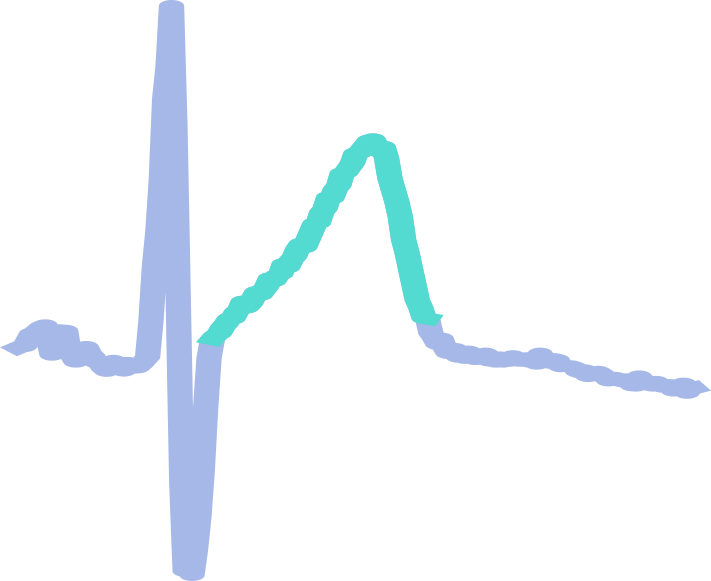
\includegraphics[height=3.5ex, valign=m]{large_peak_ecg.png}) or "\textit{I am searching for the QRS complex, that looks like a} \texttt{sharp peak followed by a sharp valley} (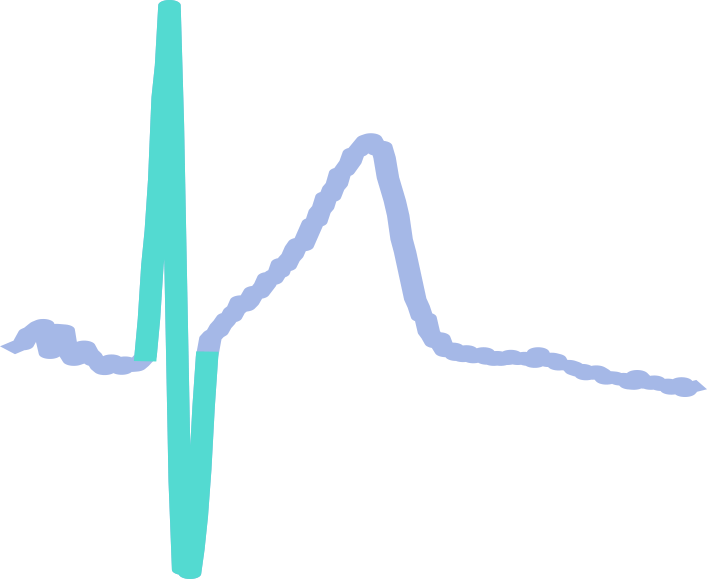
\includegraphics[height=3.5ex, valign=m]{high_peak_ecg.png})". From this textual description of patterns, one can associate words with specific properties, such as \texttt{peak} can be related with \textit{slope} and \texttt{high} related with \textit{amplitude}.
\par
The text mining domain already has available well known approaches to search for specific words or patterns with text queries in traditional text editing softwares. \gls{regex} are an example of such querying mechanisms. Other existing mechanisms rely in keyword-based queries, such as the \textit{Google} search toolbar, which sorts web-pages according to how these match the set of keywords written. These are examples of the flexibility we find in tools available for query-based text search mechanisms. We imagined such tools could also be beneficial for time series query-based pattern search tasks.
\par
In this chapter, we provide evidence that it is possible to use such reasoning with time series and propose solutions that promote higher flexibility, cognitive speed, and expressiveness in searching for patterns in time series as we would typically do with text. As presented in Figure \ref{fig:language_topics}, two main strategies are proposed: (1) Synthatic Search on Time Series (\gls{ssts}) and (2) \textit{Quo} -\textit{where}- On Time Series (\gls{quots}). The first explains how to perform query-based search on a symbolic representation of the signal. A novel symbolic representation is introduced and the usage of \gls{regex} is proposed to search for patterns directly in this symbolic representation. We also show how this representation can be used in time series classification tasks with Human Readable Time Series (HeaRTS). The second method that is proposed uses a feature-based representation of the signal, being each feature assigned to one word, which can be used with additional \textit{operators} to search for the desired patterns with natural language.
\par
The chapter will start by detailing how \gls{ssts} works, more specifically the symbolic conversion and the search process. In addition, \gls{hearts} will be explained, namely how to use \gls{ssts} and its symbolic representation to find differences between time series and ultimately be used towards interpretable classification tasks. Finally, this chapter ends with \gls{quots} and how the analyst can use feature-words (keywords) with operators to search for patterns on time series more expressively and with words.




%In terms of morphology, many attributes can be extracted from the visual perception of the signal, such as rising and falling slopes, concavity, direction, amplitude thresholding, frequency, time, and amplitude range of a slope, among others. For instance, we can identify positive peaks by finding a rising slope followed by a falling slope, which is precisely the mechanism developed in Horowitz \textit{et. al.} for peak detection in electrocardiography~\cite{Horowitz}.
%\par
%We can think of this morphological description in terms of characterization using features. These features can either be used to transform the signal into a symbolic representation, in which each sample is converted to a symbol, or a feature-based representation, in which a \textit{word-feature series} characterizes the time series for a specific property. 
%\par



\section{Syntactic Search on Time Series}

\begin{figure}
\centering
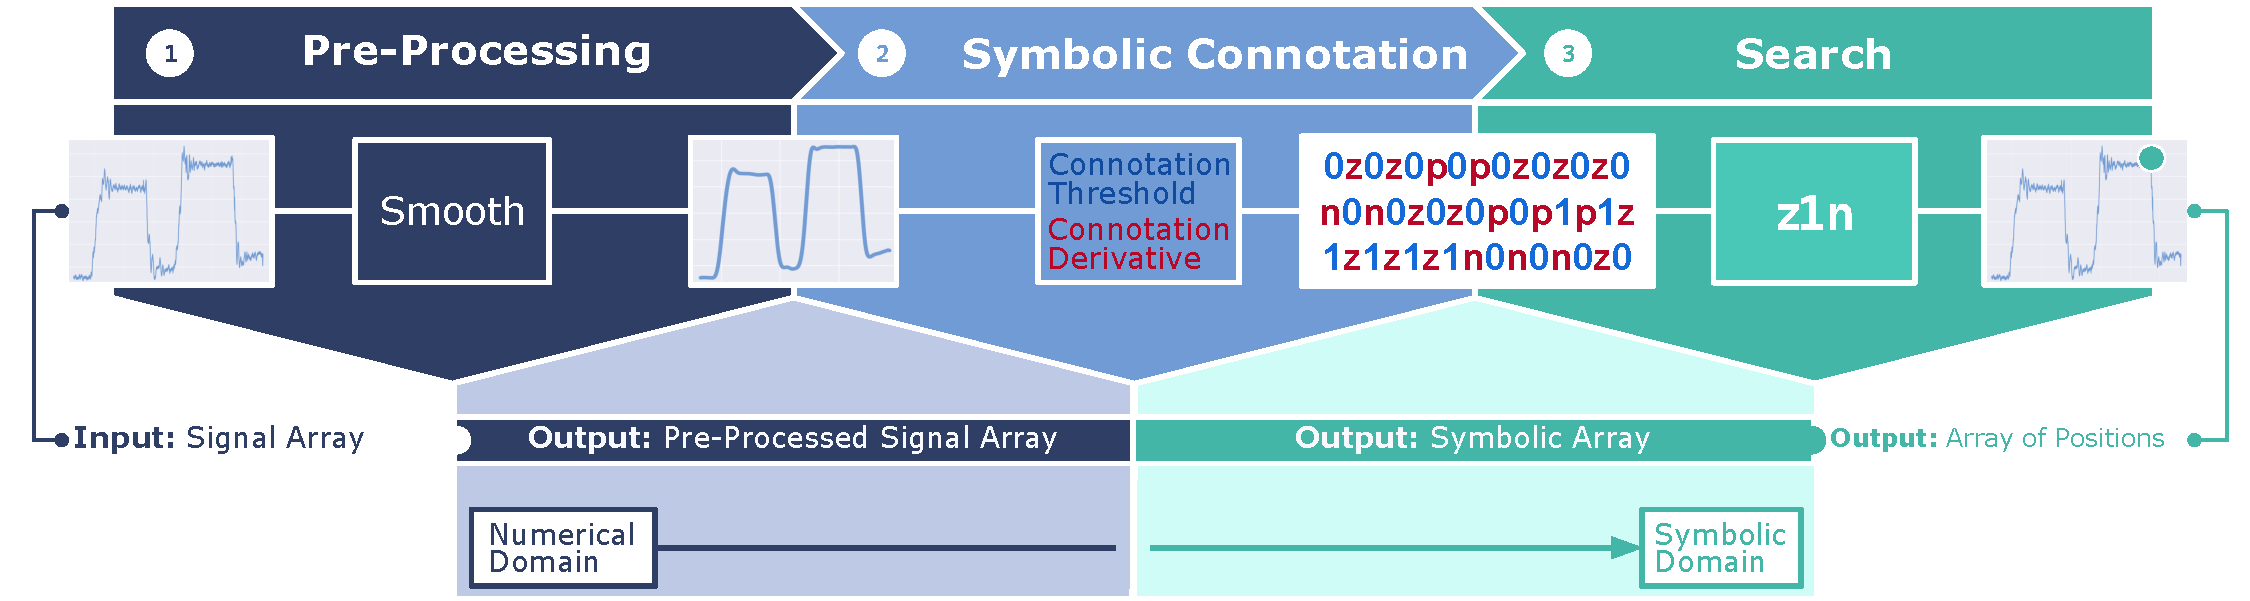
\includegraphics[width=\linewidth]{ssts_intro.pdf}
\caption{\gls{ssts} modular architecture: the proposed system is divided into three main modules - pre-processing, symbolic connotation, and search. This Figure also provides an example of the sequence of changes that occur in each step.}
\label{fig:ssts_intro}
\end{figure}

In Chapter \ref{cha:theory} was presented the well-known \gls{sax}, which is a symbolic representation of the time series based on its amplitude distributions. With \gls{sax}, query with text was not considered, but \gls{ssts} takes inspiration from this symbolic transformation by including additional attributes besides amplitude, such as the derivative, speed of the derivative, etc... (as will be listed further). Each property characterizes each sample of the signal. The combination of these attributes into a sequence of primitives is a symbolic characterization of the signal that enables the use of text-based querying mechanisms, such as \gls{regex}, to search the desired patterns. Overall, the proposed tool benefits from the visual interpretation made by the analyst and provides \gls{ssts} to express it as a \gls{regex}. 
\par
The proposed tool, \gls{ssts}, is structured in three stages:

\begin{itemize}
\item \textbf{pre-processing} - prepare the signal to highlight the desired patterns and ease the search process;
\item \textbf{connotation} - a symbolic representation of time series into a set of primitives that give information about the shape and attributes of the time series over time and is governed by a set of grammatical rules;
\item \textbf{search} - a parser (\gls{regex}) to search for patterns in the symbolic representation. Both \textit{pre-processing} and \textit{connotation} steps rely on \textit{tokens} to call specific methods. 
\end{itemize}

The next sections explain each step of the \gls{ssts} process and will be accompanied by an example to elucidate how it works. The represented signal is the \textit{z} axis of an \gls{acc} placed on the wrist of a subject while performing a rotating task at different angles. The purpose of this example is to find the time intervals where the plateaus above a certain threshold begin to decrease. Each step of this problem's resolution is shown in Figure \ref{fig:ssts_intro} and will be thoroughly explained throughout the next sections. We take the liberty to start introducing some of the processing tokens ( $Sm$ is the smooth function, $A$ is the Connotation Threshold and $D1$ is the Connotation Derivative) to give a base complete example of the usage of the \gls{ssts}.


\subsection{Pre-Processing - Preparing the Data}

The \textit{pre-processing} stage is responsible for preparing the signal, either by removing noise that arises from several sources or adjusting the signal so that the information is unveiled. Traditional pre-processing methods, such as a pipeline of linear filters, moving window average filters and statistical de-noising or re-sampling techniques, are typical procedures to prepare the signal for further tasks \cite{preProcessing}. The current approach uses a symbolic representation of these techniques, in which each is represented by its corresponding \textit{token}, which can be a symbol or a function name. In order to manage the \textit{pre-processing} tasks, a string containing a set of tokens and their corresponding arguments is written by following the polish notation \cite{polishNotation}, in which the token precedes the corresponding argument(s), and each element is separated by a white-space character. The available pre-processing methods to be used with \gls{ssts} are presented in Table \ref{tab:preprocess}.
\par
In the example of Figure \ref{fig:ssts_intro}, the \textit{pre-processing} step uses the following string: \texttt{$Sm$ 500}, which indicates that a smooth filter using a sliding window with a size of \textit{500} samples is applied to the signal. The resulting signal is showed under its original form. The selected area in the Figure \ref{fig:ssts_intro} represents the segment of the signal that will be represented in subsection \ref{subsec:symbolic_connotation}.

\begin{center}
\begin{table}
	\centering
    \setlength{\tabcolsep}{3pt}
	\renewcommand{\arraystretch}{1.5}
	\caption{List of common \gls{ssts} pre-processing operators. As input parameters, \textit{s} is the signal, \textit{fc} is the cut-off frequency and \textit{win\_size} is the size of the window used (number of samples). The linear filters (HP, BP, and LP) have a default order of 2}
	~\\~
	\label{tab:preprocess}
	\begin{tabular}{lcP}
        \toprule[0.5mm]
		Name & Input Parameters & Description\\
        \midrule[0.3mm]
		HP & (\textit{fc}) & Linear high-pass filter with cut-off frequency \textit{fc}\\
        \midrule
		BP & (\textit{fc1}, \textit{fc2}) & Linear band-pass filter with cut-off frequencies \textit{fc1} and \textit{fc2}\\ 
        \midrule
 		LP & (\textit{fc}) & Linear low-pass filter with cut-off frequency \textit{fc}\\
        \midrule
        abs & none & Modulus of signal - $|T|$\\
        \midrule
        Mag & none & Magnitude - $|T| = \sqrt[]{T_0^2 + T_1^2 + T_2^2}$\\
        \midrule
        Sm &  (\textit{win\_size}) & smoothing of \textit{T} by a moving average window filtering technique of size \textit{win\_size}\\
        \midrule
        $Z_{norm}$ & (\textit{s}) & z-normalize the time series $\overline{T} = \frac{T-\bar{\mu_T}}{\sigma_T}$, being: $\overline{T}$ the normalized signal, $\bar{\mu_T}$ the signal's mean and $\sigma_T$ the standard deviation of the signal\\
        \midrule
        | & N.A. & Separates the pre-processing methods applied to multiple signals or multiple processing of the same signal\\
        \bottomrule[0.5mm]
 	\hline
	\end{tabular}
\end{table}
\end{center}

\subsection{Connotation - The Symbolic Time Series}
\label{subsec:symbolic_connotation}


\begin{figure}
\centering
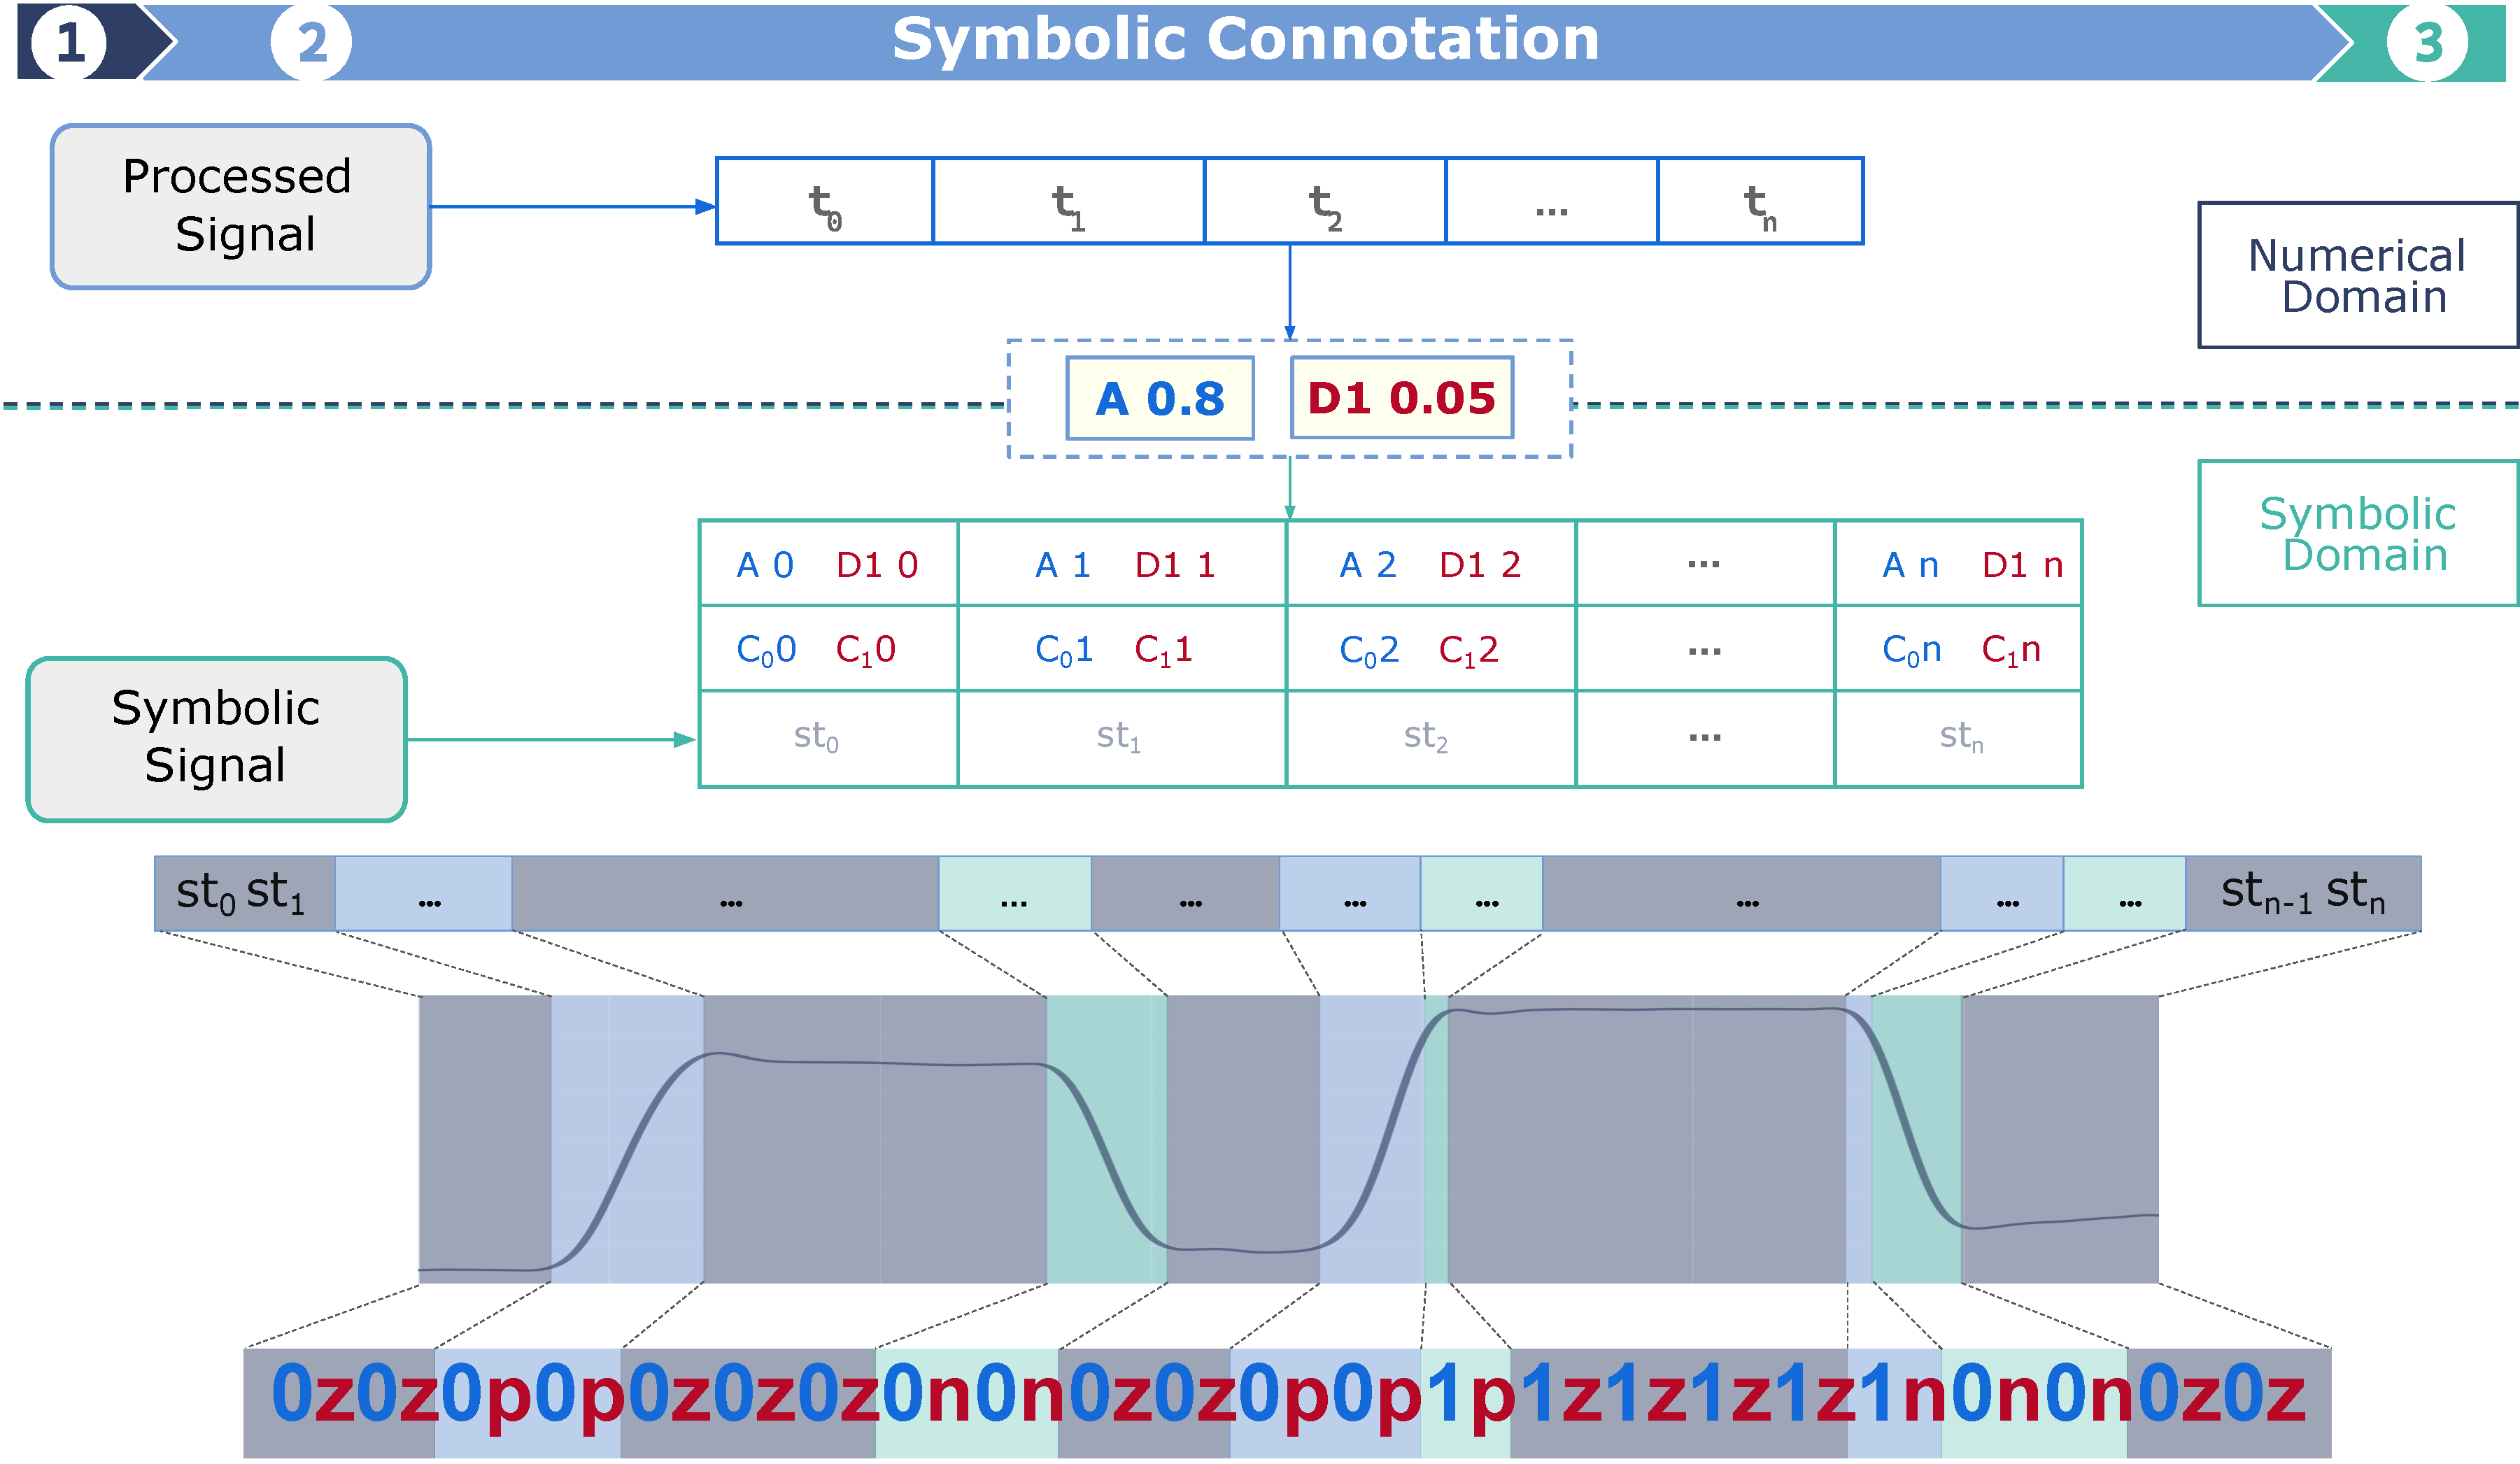
\includegraphics[width=\linewidth]{ssts_connotation_step.pdf}
\caption{Here are highlighted the second stage of the process. It is the moment the signal is transformed from the numerical domain to the symbolic domain. $A$ represents the amplitude method (blue) while $D1$ is the first derivative (red). The exemplified signal plus the symbolic translation are presented.}
\label{fig:ssts_connotation}
\end{figure}

In semiotics, it is stated that the connotative aspect of an image or a sign corresponds to the extraction of meaning (sometimes called the \textit{second meaning}), by the personal interpretation of its traits and characteristics \cite{connotation}. The \textit{connotation} step is the same connotative aspect but in this case, instead of a regular image, it is a time series. We follow the reasoning that the interpreter (the analyst) has made his analysis of the time series and retrieved the necessary information to search for the desired patterns. 
\par
The symbolic \textit{connotation} step generates a sequence of \textit{characters} by extracting properties of the signal that are based on a conversion rule that the user defines. Each of these conversion rules is designated a \textit{connotation} method. These are responsible for converting each sample of the signal into a \textit{character} or group of \textit{characters} that represent the state of the sample for that conversion rule (e.g. if the time series sample has a negative derivative, it will have the character \texttt{negative}). Each of the \textit{connotation} methods is related to specific attributes of the time series that are considered relevant for the search procedure. The string that results from this step is therefore a symbolic representation of the strictly necessary attributes of the signal that are best suited to specify a pattern match. Note that this process is decided by the analyst.
\par
The string can be based on a single connotation method or a combination of multiple ones. In addition, the \textit{connotation} process also handles multidimensional time series, in which cases the string is a combination of \textit{connotation} methods corresponding to each time series, returning a group of \textit{characters} for each of its samples.
\par
Following the previous description, we recall the general text definitions from Section \ref{subsec:text_abstraction} and associate these with \textit{connotation} step's output. Each sample of the time series, $T=(t_1, t_2, ..., t_n)$,  is converted into a \textit{character} from this \textit{connotation} alphabet ($char_C$), generating a symbolic time series, $ST = (st_1, st_2, ..., st_i, ..., st_n)$, in which $st_i = char_C$. A \textit{character} is any unit symbol from the connotation alphabet ("Group of Symbols" in Table \ref{tab:connotation}). When the analyst selects more than one \textit{connotation} method to transform the time series $T$, each sample of $T$ is converted into the corresponding \textit{characters}, one for each alphabet of each \textit{connotation} method applied, resulting in: $st_i =$ $<char_{C1}><char_{C2}><...><char_{Cc}>$, being $ char_{Cc}$ the $c^{th}$ \textit{connotation} method applied. In case $T$ is a multidimensional time series, the symbolic time series (MST)' samples from each time series are grouped $MST =$ ($<st_{1,1}><...><st_{1,k}>,..., <st_{n,1}><...><st_{n,k}>$).

The set of connotation methods can be defined by the user and added as needed. A base list of connotation methods and the corresponding symbols/tokens used for the examples presented are listed in Table \ref{tab:connotation}.

\begin{table}[h!]
	\centering
	\caption{List of base \gls{ssts} connotation operators. The input parameters are \textit{s}, which represents the input signal and \textit{thr}, which defines the threshold percentage value of the amplitude range of the signal ($max(s) - min(s)$) for a given connotation method. The operator that separates the connotation methods applied to multiple signals or multiple representations of the same signal is the vertical bar "\textbf{|}".}
	~\\~
	\label{tab:connotation}
   \setlength{\tabcolsep}{3pt}
   \renewcommand{\arraystretch}{1.5}
   \begin{tabular}{
   c M{0.1\linewidth} M{0.2\linewidth} E} 
   \toprule[0.5mm]
		Name & Input Parameters & Group of Symbols & Description\\ \midrule[0.3mm]
		 A & (\textit{s}, \textit{thr}) & ["1","0"] & Amplitude comparison, If $t_i$ > \textit{thr}*($t_{max} - t_{min}$), $t_i$ is "1", else $t_i$ is "0"\\ 
         \midrule   
		D1 & (\textit{s}, \textit{thr}) & ["p", "n", "z"] & Derivative of signal \textit{s} (\textit{s'}). If $t'_i$ > \textit{thr}, $t'_i$ is 'p'; elif $t'_i$ < \textit{- thr}, $t'_i$ isn't; else, $t'_i$ is "z". \\ 
        
        \midrule
        
        D2 & (\textit{T}, \textit{thr}) & ["D", "C", "z"] & Second derivative of signal \textit{T} (\textit{T"}). If $t"_i$ > \textit{thr}, $t"_i$ is 'D'; elif $t"_i$ < \textit{- thr}, $t"_i$ is 'C'; else, $t"_i$ is "z". \\ 
        
        \midrule
        
 		AD & (\textit{s}, \textit{thr}) & ["1", "0"] & Determinates if amplitude from a minimum to a maximum and vice-versa is superior to \textit{thr}. If so, $t_i$ is "1", else, $t_i$ is "0". \\  
 		
 		\midrule
 		
 		SA & (\textit{s}, \textit{thr}) & ["r", "R", "f", "F"] & Amplitude of a slope segment. The characters are case sensitive, being \textbf{\textit{r}} for a low rise and \textit{\textbf{R}} for a high rise. The same for falling (\textbf{\textit{F}} or \textbf{\textit{f}}). \\
 		
 		\midrule
 		
 		SS & (\textit{s}, \textit{thr}) & ["r", "R", "f", "F"] & Speed of the signal measured by the amplitude on the first derivative. When the sample is quicker than the threshold it is converted to "R" - quick rise or "F" - quick fall, whereas when slower it is converted to "r" - slow rise or "f" - slow fall.\\
        \bottomrule[0.5mm]
	\end{tabular}
\end{table}


The symbolic connotation step of the exercise of Figure \ref{fig:ssts_intro} demonstrates the latter formalism. In Figure \ref{fig:ssts_connotation}, the processed signal is decomposed in a symbolic sequence by two connotation methods: amplitude (blue) and derivative (red). The first implies that the sample values superior to the threshold \textit{\textbf{0.8}} will be "1", while the rest turns "0", whereas the second gives the value "p" when the signal is increasing, "n" when decreasing and "z" when stationary with a threshold of \textit{\textbf{0.05}}. Each of the samples of the signal is converted into the primitive ($st_1...st_n$) which is the alternate association of the two connotation methods. The approximate result is illustrated by the bottom string, in which can be seen the alternation property and what it translates. The representation made using these two methods is expected to be necessary to ease the search procedure.

\subsection{Expressive Syntactic Search}

\begin{figure}
\centering
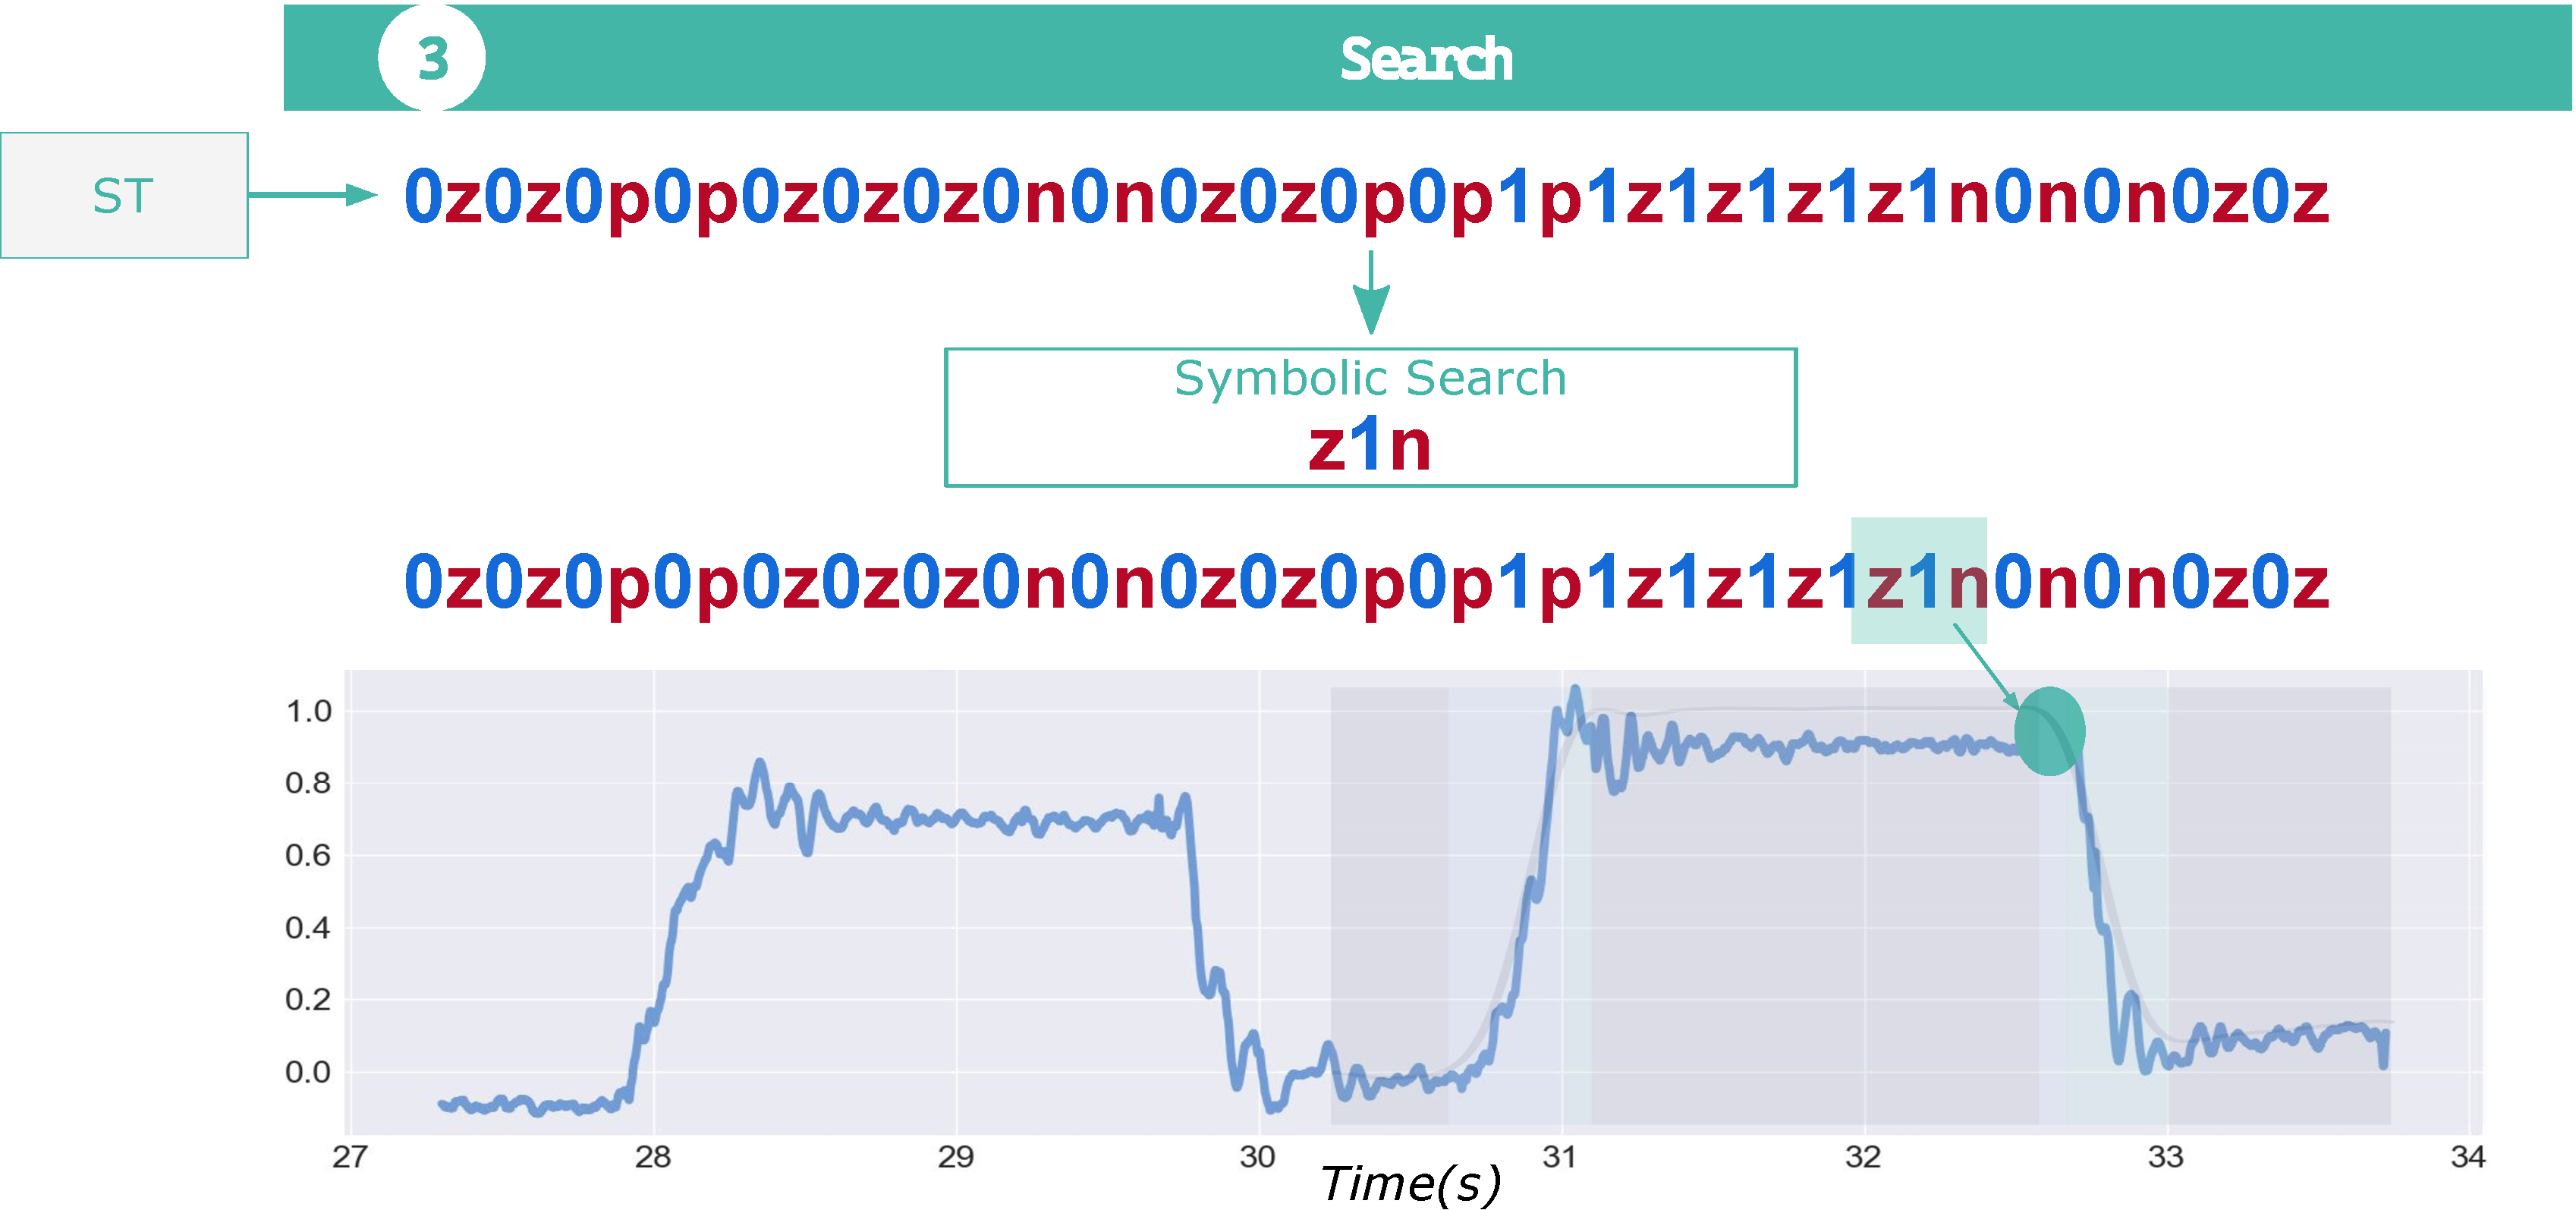
\includegraphics[width=\linewidth]{ssts_search_step.pdf}
\label{fig:ssts_search}
\caption{Step 3 of \gls{ssts}. Specific \textit{subsequences} of the time series can be searched with a \gls{regex}. In this case, the search is to find the moment a \texttt{plateau} starts to fall, which is found with the \gls{regex} \texttt{z1n}. Blue are the symbols for amplitude and red for the first derivative.}
\end{figure}

The last step of the process involves searching for the desired pattern in the generated symbolic time series with a \gls{regex}. This string is governed by the rules of \gls{regex} from the \textit{alternative \gls{regex} Python module} \cite{rgxPy} and benefits from all the functionalities and meta-characters typically used with this tool, which can be recalled from Chapter \ref{cha:theory} (see Section \ref{subsec:regex_theory}). The search procedure returns the intervals at which positive matches occurred. It is relevant to note that it has been decided to use \gls{regex}, although any other parser, conveniently combined with the previous steps, might be used for the same purposes.
\par
In the example of Figure \ref{fig:ssts_intro}, the purpose is to determine when a plateau superior to \textit{80 \%} of the amplitude range of the signal starts to fall. The symbolic time series matches this moment when a the sequence of characters starts with a \texttt{1} (\textit{time series is higher than the 80 \% threshold}) and is followed by  the sequence \texttt{zn} (\textit{a sequence of stationary  to falling}). The \gls{regex} used for the search is precisely \texttt{z1n}, which indicates that the signal, at some point superior to the threshold will start to decrease, as presented in Figure \ref{fig:ssts_search}.
\par
In the next Chapter we will show several applications of this method for pattern search tasks. Next, we present how  to use it for classification purposes.

\section{Towards Interpretable Time Series Classification with SSTS}

\begin{figure}[b]
\centering
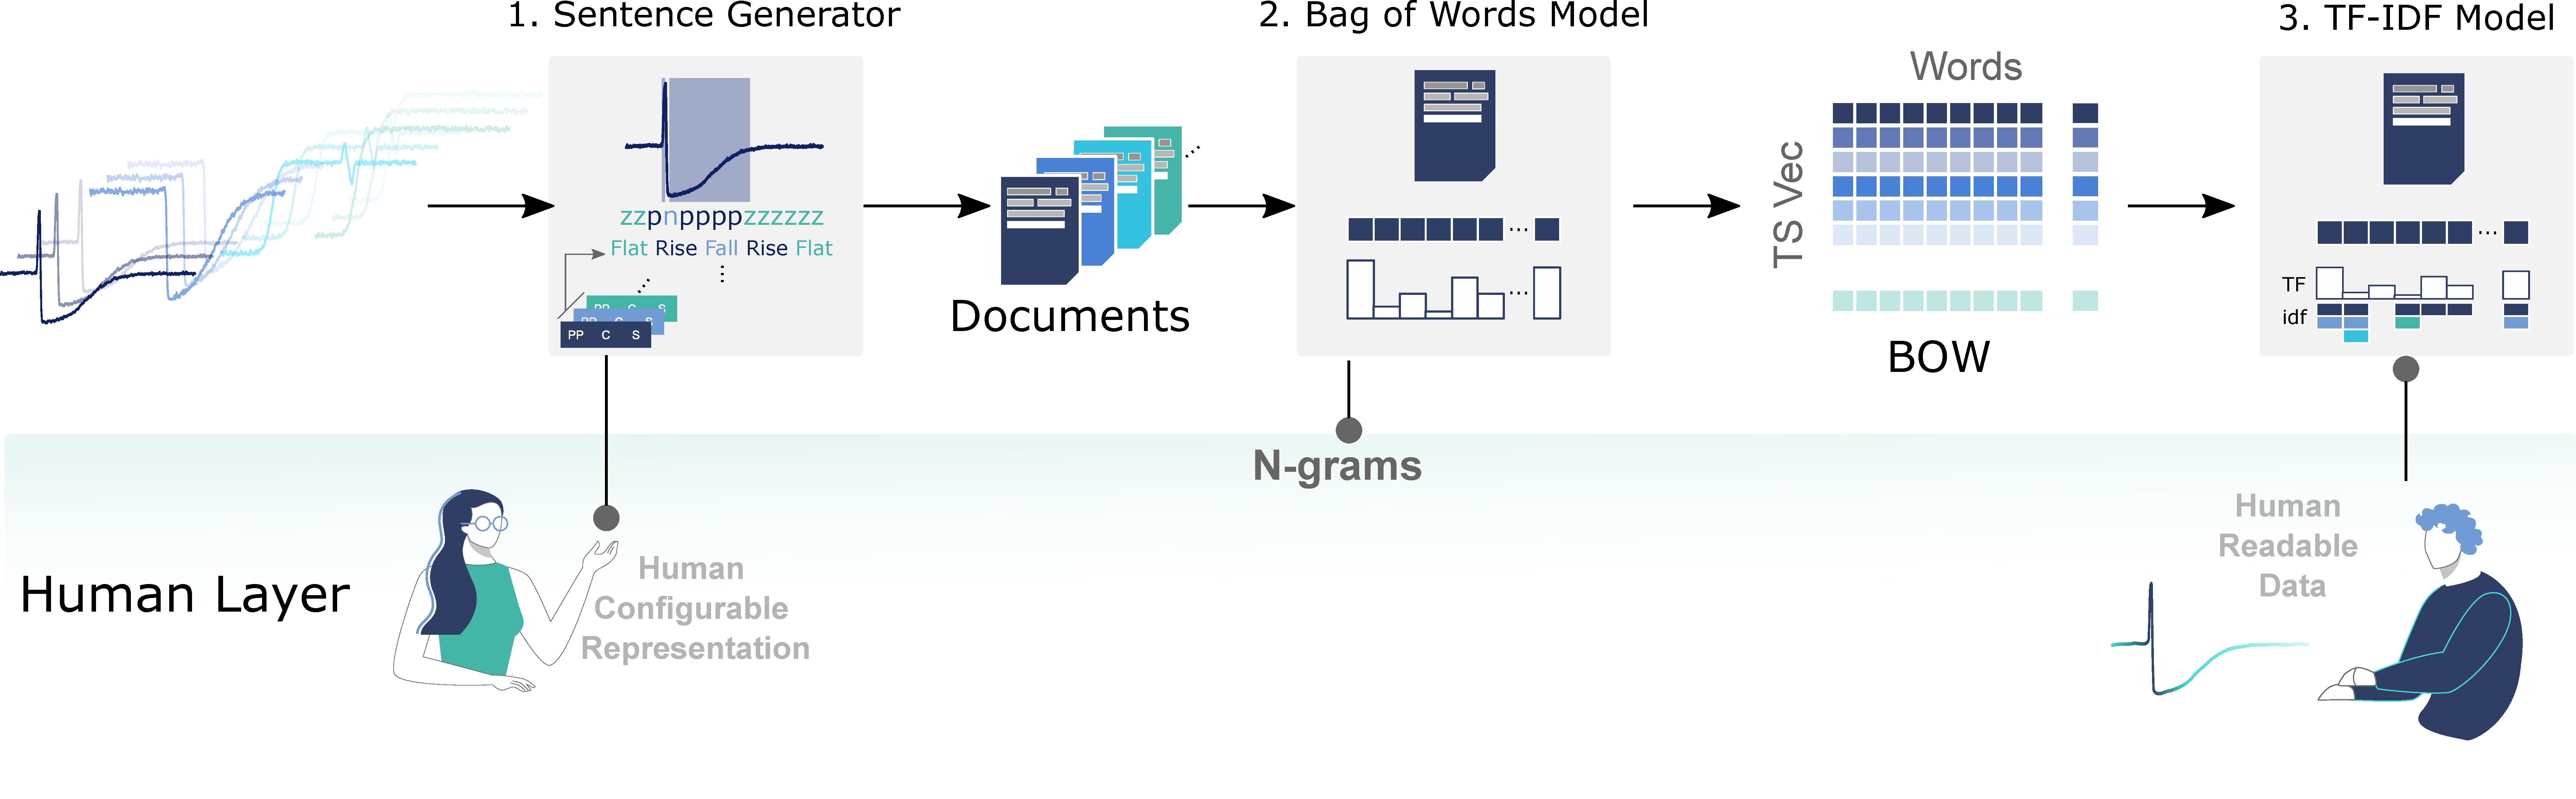
\includegraphics[width=\linewidth]{overall_interpretable.pdf}
\label{fig:overall_interpretable}
\caption{Steps of transforming time series into documents and corresponding \gls{bow} and \gls{tfidf} matrices for posterior classification. The steps are (1) \textit{sentence generation}: all time series are converted to time series \textit{documents} multiple \gls{ssts} queries (e.g. \texttt{Flat}, \texttt{Rise} and \texttt{Fall} from the derivative \textit{connotation}); (2) \textit{bag of words model}: each document is converted to a vector with the frequency of words in that document; and (3) \textit{tfidf model}: transforming the \gls{bow} to \gls{tfidf} and possibly searching for relevant segments of the time series. The human layer shows where the human can apply his/her knowledge, namely selecting the \gls{ssts} queries and interpreting the highlights on the signal.}
\end{figure}

The ability to transform a time series into a meaningful symbolic representation makes the usage of text-mining tools available for time series analysis. Profiting from such methods can result in different outcomes that can complement the ones resulting from current strategies, improve results or even open novel pathways for further research experiments in this domain.

We propose to use the existing text-mining knowledge on this novel representation for time series classification. In order to perform a class separation, differences and similarities have to be highlighted, and this is also possible to be done with text. In the text mining domain, the differences between text \textit{documents} are traditionally computed with a feature extraction process on text, such as \gls{bow} or \gls{tfidf}, returning a statistical representation of the words or n-gram. \textit{Documents} with different words and/or sequences of words will have different weights on these models, which are used to perform a class separation on the \textit{documents}. We take inspiration from this process and apply it to time series. For instance, the following time series 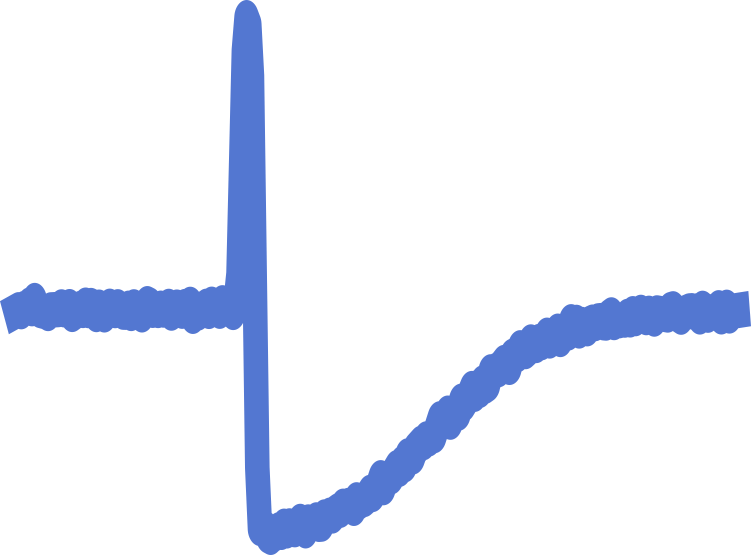
\includegraphics[height=2.5ex, width=3.5ex, valign=m]{trace1.png} can be very broadly translated into \texttt{Flat Rise Fall Rise Flat} or \texttt{Flat Peak Valley Flat}, while the following signal 
\includegraphics[height=2.5ex, width=3.5ex, valign=m]{trace_2.png} would be translated into \texttt{Flat Fall Rise Flat} or \texttt{Flat Valley Flat}. This type of description is easily performed with \gls{ssts}, as showed on Figure \ref{fig:SSTS_example}. Figure \ref{fig:overall_interpretable} shows the main steps to perform a transformation of the time series into a \gls{bow}/\gls{tfidf} model that can be used with a classifier. 

In this section, we explain each step of the proposed strategy to perform time series classification based on a textual description with \gls{ssts}. The fact that the time series is translated into text also provides a layer of readability and interpretability to the data, as we will explore throughout this section as well.

%
%The proposed method conceptually developed based on text mining techniques abstracts how a time series can be structured in a linguistic representation, similar to how the human would describe a time series with words. In order to introduce the reader to this abstraction and representation, we explain how we use \textit{SSTS} to make this abstraction.
%
%
%
%The transcription results in sequences of \textit{characters}. Specific \textit{characters} sequences are translated into \textit{words}.\\
%
%\textit{\textbf{Definition 2.5}} A \textit{word} is a sequence of \textit{characters}. \textit{SSTS} has the \textbf{search} step which provides a way of extracting specific patterns with \gls{regex} queries. We pre-defined a set of search queries that correspond to specific words, such as \textit{rise}, \textit{fall}, \textit{peak}, \textit{valley}, etc.... These words can be associated with a single character (e.g. rise = \textbf{\textit{p+}}) or a combination of them (e.g. peak = \textbf{\textit{p+[z]n+}}). Examples of common matches are presented in Figure.
%
%This set of words belongs to a \textit{vocabulary}.\\
%
%\textit{\textbf{Definition 2.6}} The \textit{vocabulary} comprehends the set of words available in a pre-defined set of \textit{SSTS} queries.
%
%The \textit{words} used can be ordered to form a \textit{sentence}.\\
%
%\textit{\textbf{Definition 2.7}} \space \space A \textit{sentence} is a set of \textit{words} or tokens organized sequentially. In this work, we create multiple sentences based on the types of \textit{connotation} methods used to transcribe the time series. In Figure \ref{fig:SSTS_example}.Bottom, a time series is translated into the \textit{sentence} \textbf{\textit{Flat Rise Fall Rise Flat}} based on a set of \textit{SSTS} queries from the derivative connotation (\textit{\textbf{p+, z+}} and \textbf{\textit{n+}}). 
%For each time series, one document is generated. 
%
%\textit{Sentences} can be added to a \textit{document}. \\
%
%\textit{\textbf{Definition 2.8}} \space \space A \textit{document} is a piece of text with a collection of words or tokens that are used to build sentences. It can be made of only one sentence or multiple ones. In this work, a \textit{time series document} will have multiple sentences as groups describing patterns. 
%Finally, the higher hierarchy in textual information is the \textit{corpus}.\\
%
%\textit{\textbf{Definition 2.9}} \space \space The \textit{corpus} is a collection of text material (group of documents). It represents a higher level of textual information. This collection is typically annotated and used for machine-learning tasks. In this case, a corpus will be represented by the set of documents that describe a time series dataset.
%
%Since this work follows the steps of \textit{NLP} strategies for document classification, we will define \textit{Bag of Words} (BoW).\\
%
%\textit{\textbf{Definition 2.10}} \space \space A BoW is a feature matrix representation of a corpus, being the feature the number of occurrences of each word, the term-frequency (\textit{tf}):
%\begin{equation}
%    tf_{t,d} = \frac{f_{t,d}}{\sum\limits_{t'\in d} f_{t',d}}, 
%\end{equation}
%
%being \textit{t} the term that exists in a document, \textit{d} the document, \textit{t'} the term that belongs to document \textit{d}.
%
%We use the BoW to vectorize the textual representation of each time series.
%
%Most of the time, \textit{n-grams} are used in addition to single words.\\
%
%\textit{\textbf{Definition 2.11}} \space \space \textit{N-grams} are a span of followed words that are counted in the BoW. It gives more context to words that are frequently followed by a specific word. As with time series we have temporal order of occurrences, this feature is very important. An example of \textit{2-gram} from the sentence \textit{Rise Flat Fall} would be \textit{Rise Flat} and \textit{Flat Fall}.

\subsection{SSTS to Generate Time Series Documents}

\begin{figure}[!h]
    \centering
    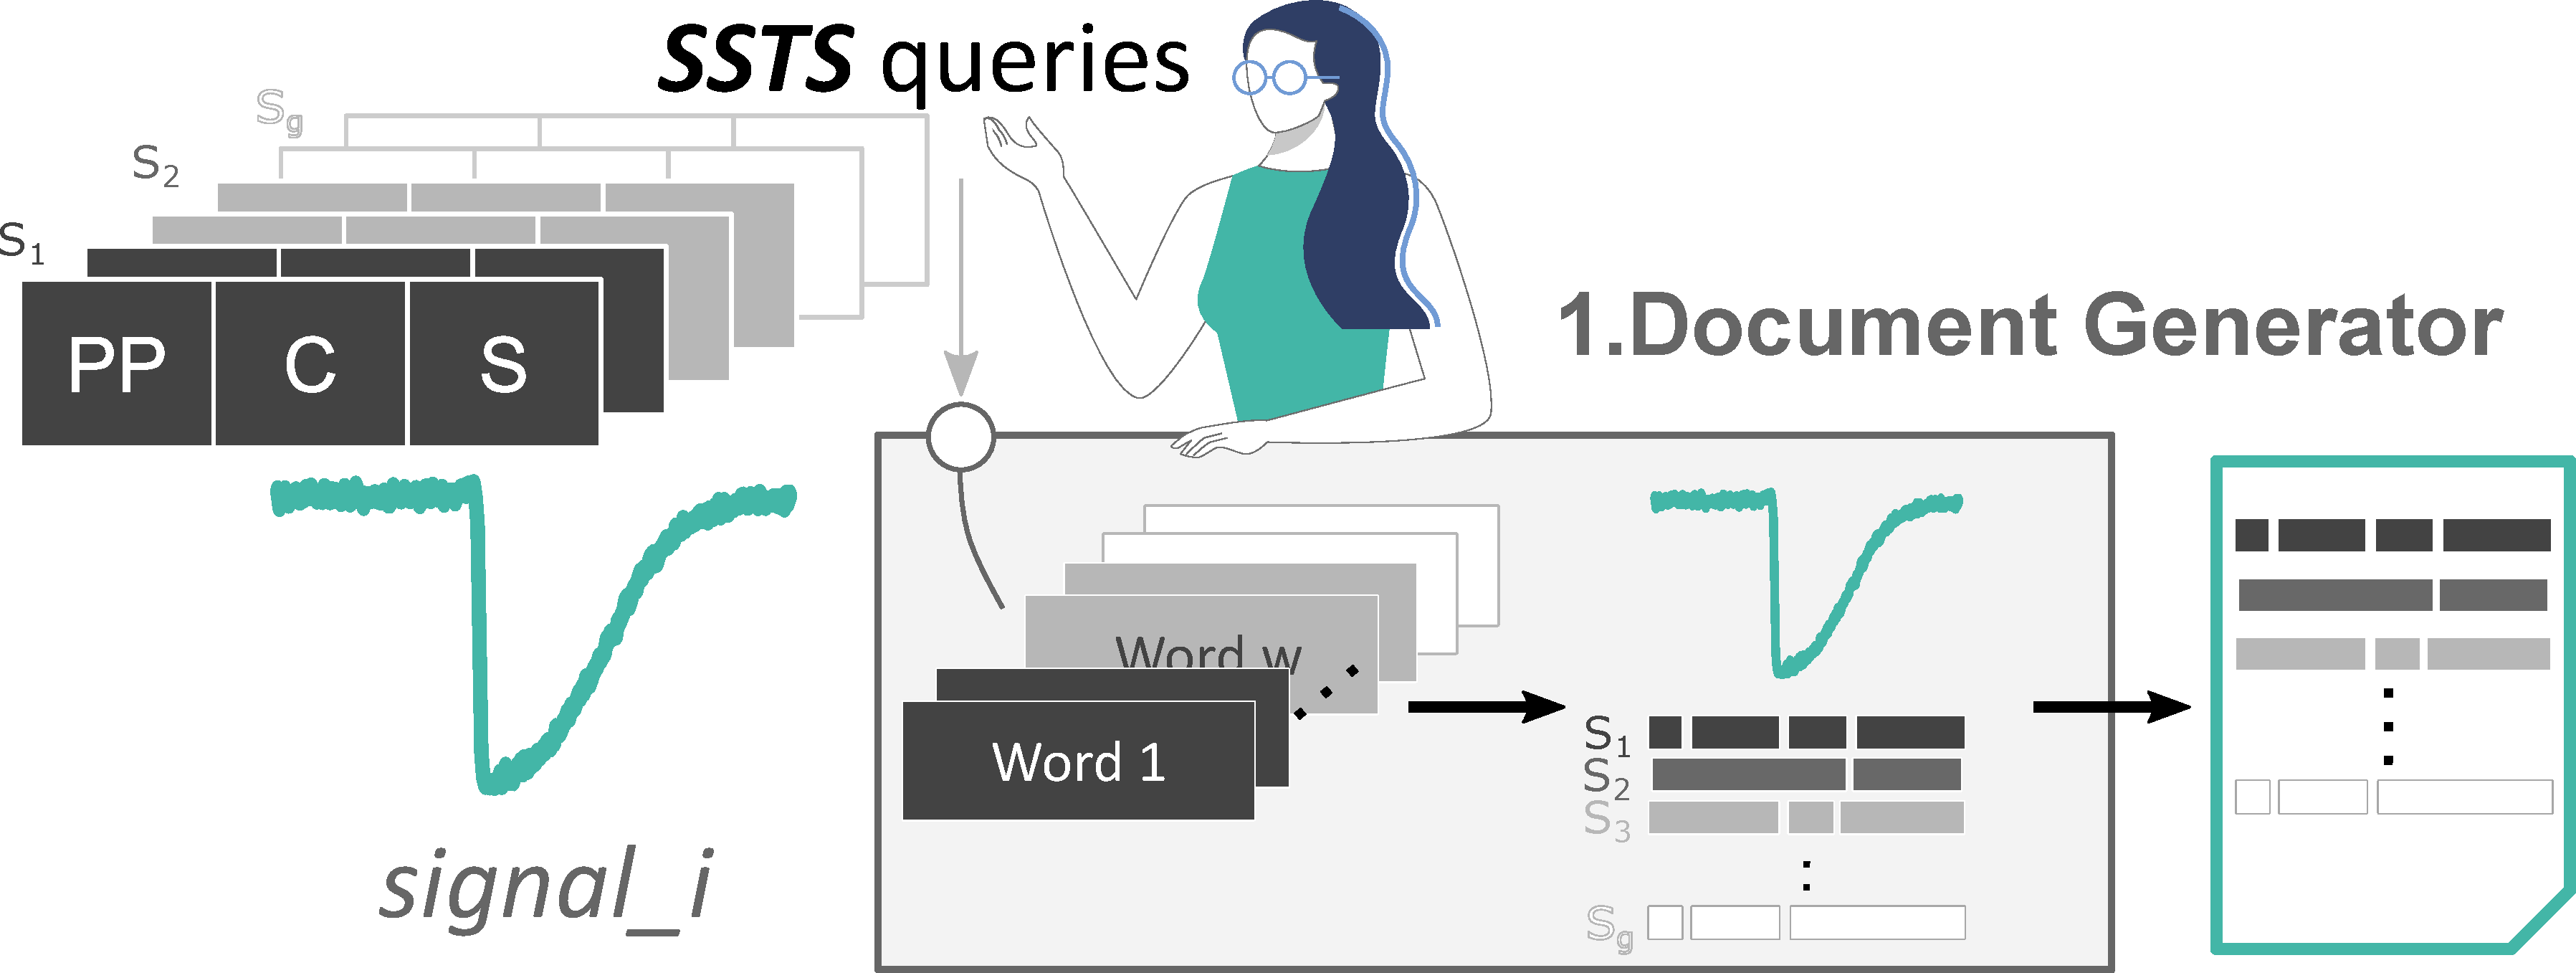
\includegraphics[width=0.85\linewidth]{interpretable_class_intro.pdf}
    \caption{Steps for the generation of sentences from a raw time series and organization as a time series \textit{document}. Here: {PP - Pre-processing, C - connotation and S - Search} are each \gls{ssts} queries used to search for the patterns and attribute the matched \textit{subsequences} to a \textit{word}. The colour tones (dark grey, light grey and white) indicate each sentence group ($S_1, S_2, ..., S_g$), which has multiple \gls{ssts} queries. The result is a \textit{document} with multiple sentences.}
    \label{fig:interpretable_intro}
\end{figure}

\begin{figure}[!h]
    \centering
    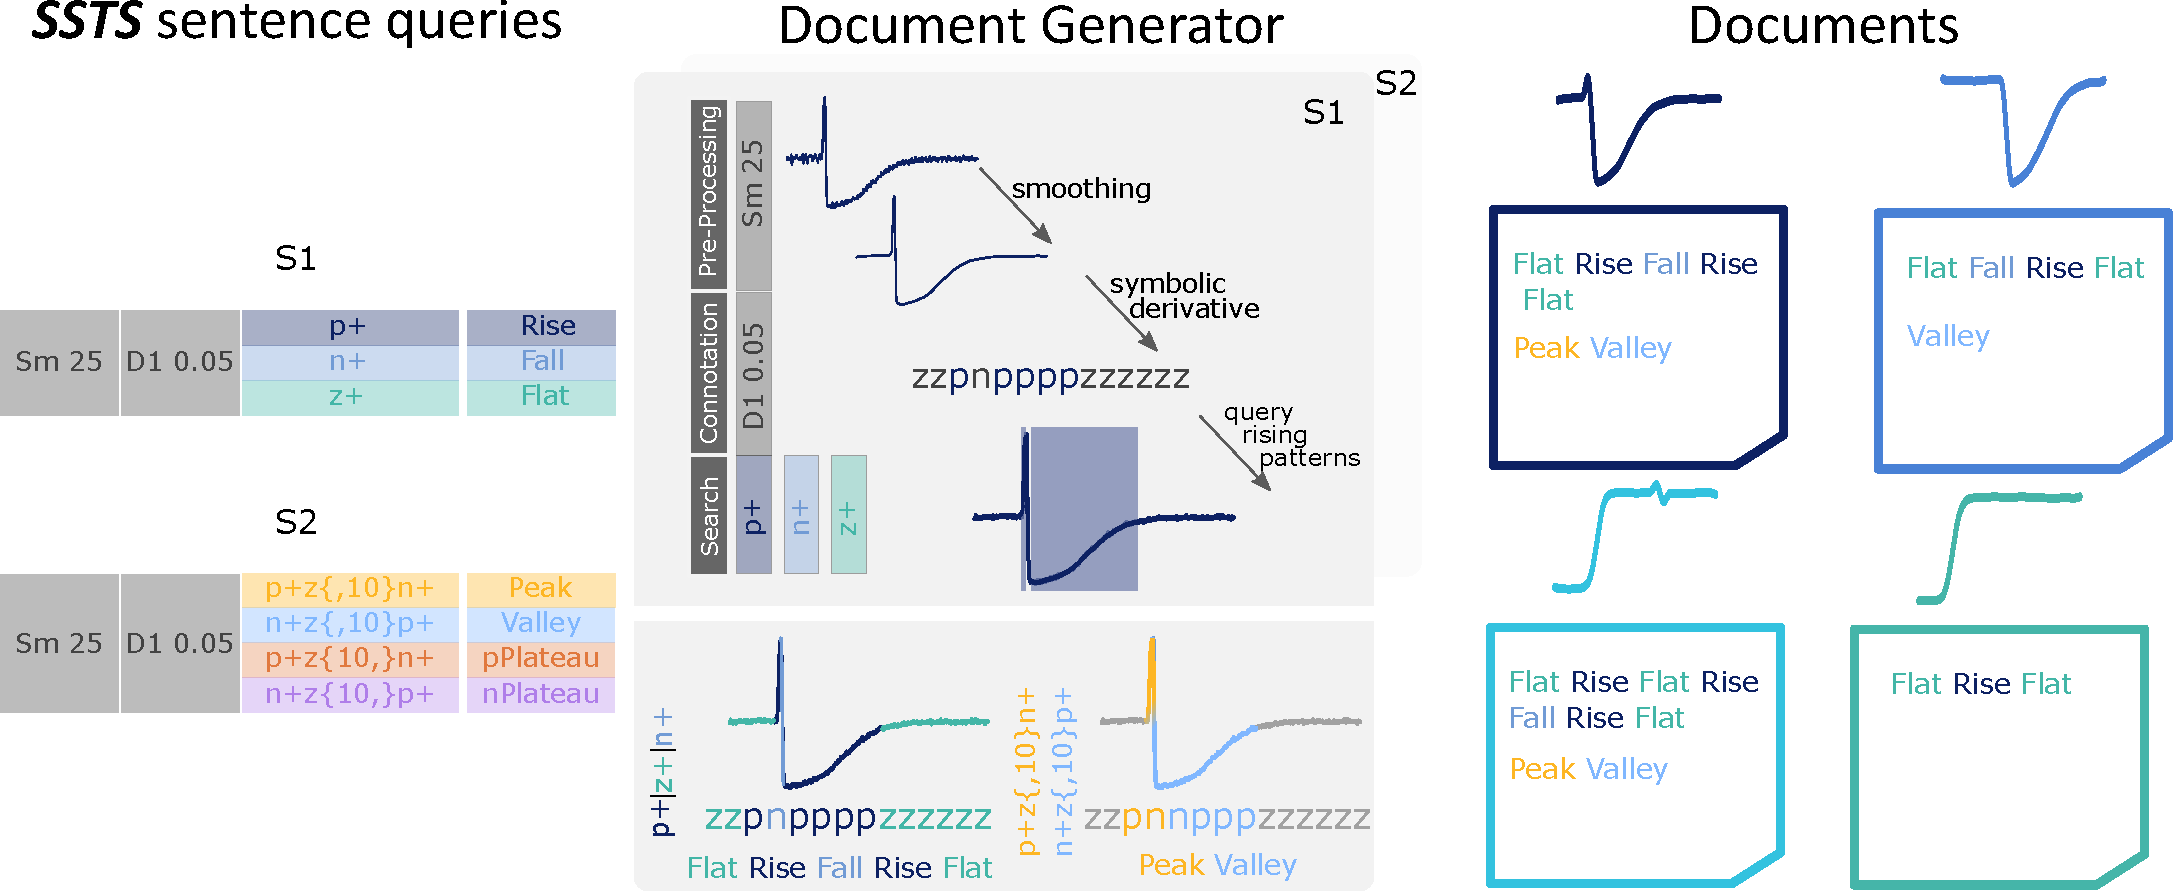
\includegraphics[width=\linewidth]{sentence_generation.pdf}
    \caption{Example of converting a time series into a time series document with \gls{ssts}. \textbf{\gls{ssts} sentence queries}: Two groups of sentences (S1 and S2) are used to extract words on a signal. Each sentence group has multiple \gls{ssts} queries, to which a word is associated (e.g. \texttt{p+} $\rightarrow$ \texttt{Rise}). \textbf{Document Generator}.Top: Using \gls{ssts} to detect the rising \textit{subsequences} (\texttt{p}) of a time series. Each step of the process is written described as follows: (1) \textit{pre-processing}: \textit{Sm} is the function \textit{Smooth} with a window size of 25 samples; (2) \textit{connotation}: \textit{D1}, indicates the first derivate, from which each sample is converted to \texttt{z} - Flat, \texttt{p} - rising and \texttt{n} falling; (3) \textit{search} - \gls{regex} \texttt{p+} searches for all sequences with one or more \texttt{p} characters. \textbf{Document Generator}.Bottom: Example of sentence generation. Using the other search queries (\texttt{p+, n+, z+}), we can find the derivative patterns and convert them into ordered words. \textbf{Documents:} the time series documents generated for each of the exemplified signals with the two sentence groups used.}
    \label{fig:SSTS_example}
\end{figure}

The generation of time series documents (See Section \ref{subsec:text_}) is made by converting samples of the signal to characters, search patterns that are tagged with specific words in which these samples are converted to, and order them by their time index. With this, the time series can be translated into sentences and be described as a text document.
\par
In order to perform this description, the words have to be associated with a specific \gls{ssts} query. Each query has the three stages of \gls{ssts} and searches for the patterns that match on the time series. The patterns that are matched are associated with the corresponding \textit{word}. As an example, the query \texttt{\{PP: Sm 25, C: D1 0.05, S: p+\}} searches for instances where the time series is increasing and attributes to these \textit{subsequences} the word \texttt{Rise}. A specific set of \gls{ssts} queries are used to build a full description of the signal dynamics in higher leveled structures, mostly related with amplitude and derivative \textit{connotations}. 

The selection of \gls{ssts} queries is made by the analyst, either using a pre-defined set of queries or creating his/her own, more appropriate for the type of signals to analyze. This is the customizable step of the process, in which the analyst can include his/her intuition.

The ability to distinguish time series with text will be as good as the descriptive richness of the generated sentences. Depending on the differences between the time series being classified, a simple description based on the sign of the signal's derivative might be enough (such as simply explaining if the signal is \texttt{Rising} or \texttt{Falling}). However, in some cases, the overall dynamic of signals might be dissimilar to other dimensions. In order to have a rich foundation to perform a sentence description of a time series, we created the set of \gls{ssts} queries presented on Table \ref{tab:ssts_queries}, grouped by sentence ($S1, S2, ...$). The table also has an example of matching the corresponding query on a real signal. We would like to highlight that these queries are not mandatory and can be adapted by the analyst or even new connotation methods and queries can be created that might make more sense for the problem being solved. In cases where the user knows exactly what kind of patterns are relevant to perform the distinction, specific patterns can be used, targeting the relevant differences. Otherwise, the existing list can be used.

\begin{table}
\begin{center}
\caption{The connotation variables, search \gls{regex} and corresponding words assigned to the pattern searched. The parameter \textit{m} indicates the size, in samples, of the difference between a peak or a plateau, \textit{thr} is the threshold for the derivative functions. Each word has a representation on an example of a signal.}
\renewcommand{\arraystretch}{1.2}
\begin{tabularx}{\linewidth}{ XXXXX } 
\toprule[1.5pt]
Sentence Group & Connotation & Search & Word & Example\\
\toprule
  \multirow{3}{1em}{S1} & \multirow{3}{3em}{D1 thr} & p+ & \textcolor{mygreen2}{Rising} &  \multirow{3}{9em}{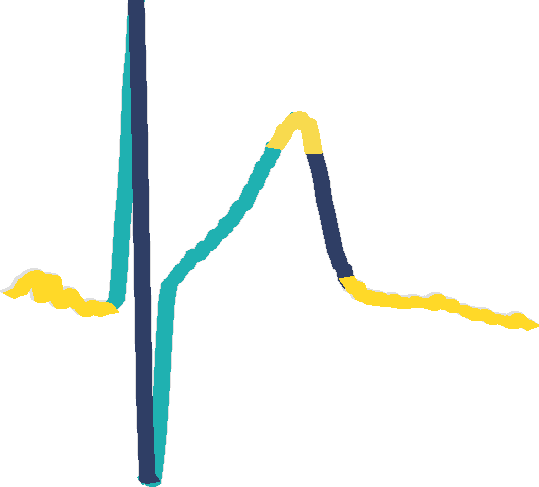
\includegraphics[height=10ex, valign=m]{ecg_overall.pdf}}\\ 
  & & n+ & \textcolor{myblue2}{Falling} & \\ 
  & & z+ & \textcolor{myorange}{Flat} & \\
\hline
 \multirow{4}{1em}{S2} & \multirow{4}{6em}{D1 thr} & p+z\{,m\}n+ & \textcolor{myblue2}{Peak} & \multirow{4}{9em}{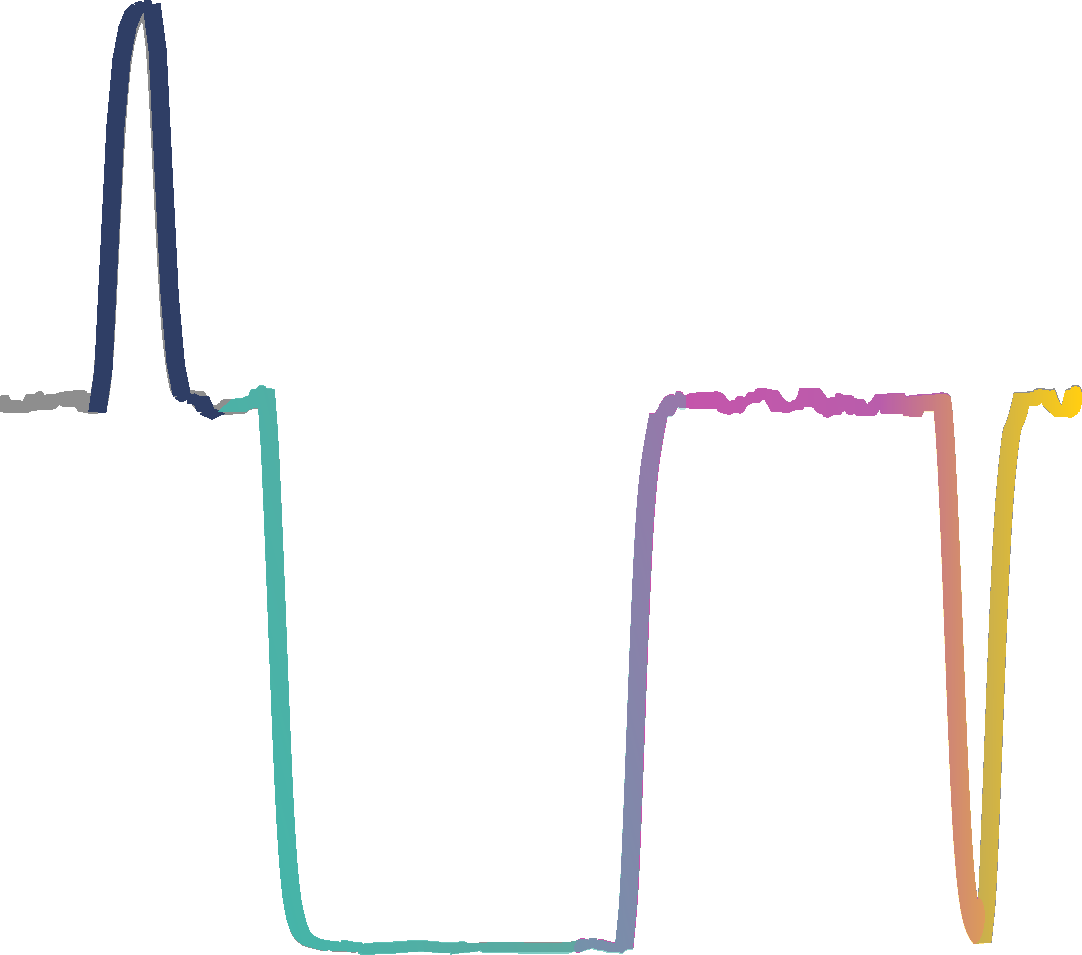
\includegraphics[height=10ex, valign=m]{peak_val_plat.pdf}}\\
 & & n+z\{,m\}p+ & \textcolor{myorange}{Valley}\\
 & & p+z\{m,\}n+ & \textcolor{mypurple}{posPlateau}\\
 & & n+z\{m,\}p+ & \textcolor{mygreen2}{negPlateau}\\
\hline
\multirow{4}{1em}{S3} & \multirow{4}{6em}{SA thr} & r+ & \textcolor{mypurple}{smallRise} & \multirow{4}{9em}{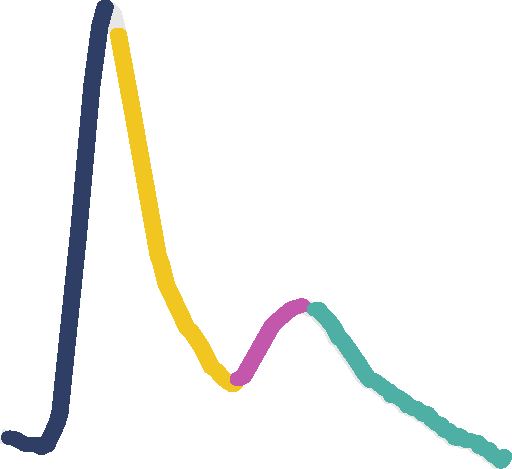
\includegraphics[height=10ex, valign=m]{abp_overall.pdf}}\\
 & & R+ & \textcolor{myblue2}{highRise}\\
 & & f+ & \textcolor{mygreen2}{smallFall}\\
 & & F+ & \textcolor{myorange}{highFall}\\
\hline
\multirow{4}{1em}{S4} & \multirow{4}{6em}{SS thr} & R+ & \textcolor{mygreen2}{quickRise} & \multirow{4}{9em}{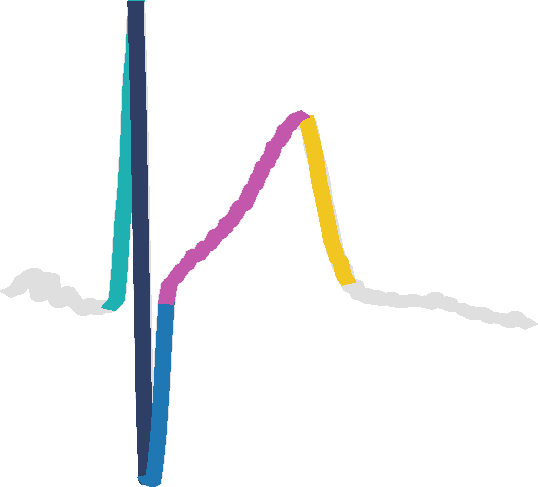
\includegraphics[height=10ex, valign=m]{ecg_overall2.pdf}}\\
  & & r+ & \textcolor{mypurple}{slowRise}\\
  & & F+ & \textcolor{myblue2}{quickFall}\\
 & & r+ & \textcolor{myorange}{slowFall}\\
\hline
\multirow{4}{1em}{S4} & \multirow{4}{6em}{A 0.5 D1 thr} & (0p)+(0z)*(0n)+ & \textcolor{mygreen2}{bottomPeak} & \multirow{4}{9em}{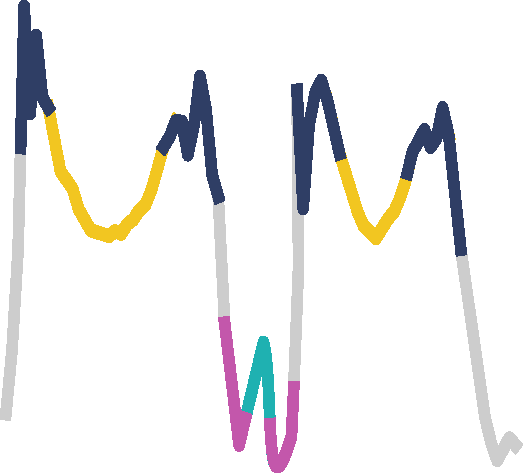
\includegraphics[height=10ex, valign=m]{example_overall_queries_4.pdf}}\\
 & & (1p)+(1z)*(1n)+ & \textcolor{myblue2}{topPeak}\\
 & & (0n)+(0z)*(0p)+ & \textcolor{mypurple}{bottomValley}\\
 & & (1n)+(1z)*(1p)+ & \textcolor{myorange}{topValley}\\
 \hline
\multirow{4}{1em}{S5} & \multirow{4}{6em}{D2 thr D1 thr} & (Dp)+ & concaveRising\\
& & (Dn)+ & concaveFalling\\
& & (Cp)+ & convexRising\\
& &(Cn)+ & convexFalling\\
\bottomrule[1.5pt]
\end{tabularx}
\label{tab:ssts_queries}
\end{center}
\end{table}
 
An example of performing this analysis on a signal is presented in Figure \ref{fig:SSTS_example}. The process highlights the usage of \gls{ssts} queries from two different groups of sentences. From the first group, the signal is analyzed in terms of derivative, matching parts of the signal where it \textit{rises, falls} or is \textit{flat}. A sentence is generated, describing it as \texttt{Flat Rise Fall Rise Flat}. The same process is done now with the second group of \gls{ssts} queries, but this time, searching for \textit{peaks, valleys, and plateaus}. A sentence is then generated based on the matches: \texttt{Peak Valley}. The same process is applied to each class of signals, being, for each signal, generated a \textit{document} with the corresponding sentences.

Having now a method to translate time series into text, we can use text mining methods directly on the \textit{documents}. Typically, text data is vectorized with the \gls{bow} or \gls{tfidf} models, a process explained in the next Section.

\subsection{Vectorization of Time Series Documents}


\begin{figure}[!h]
    \centering
    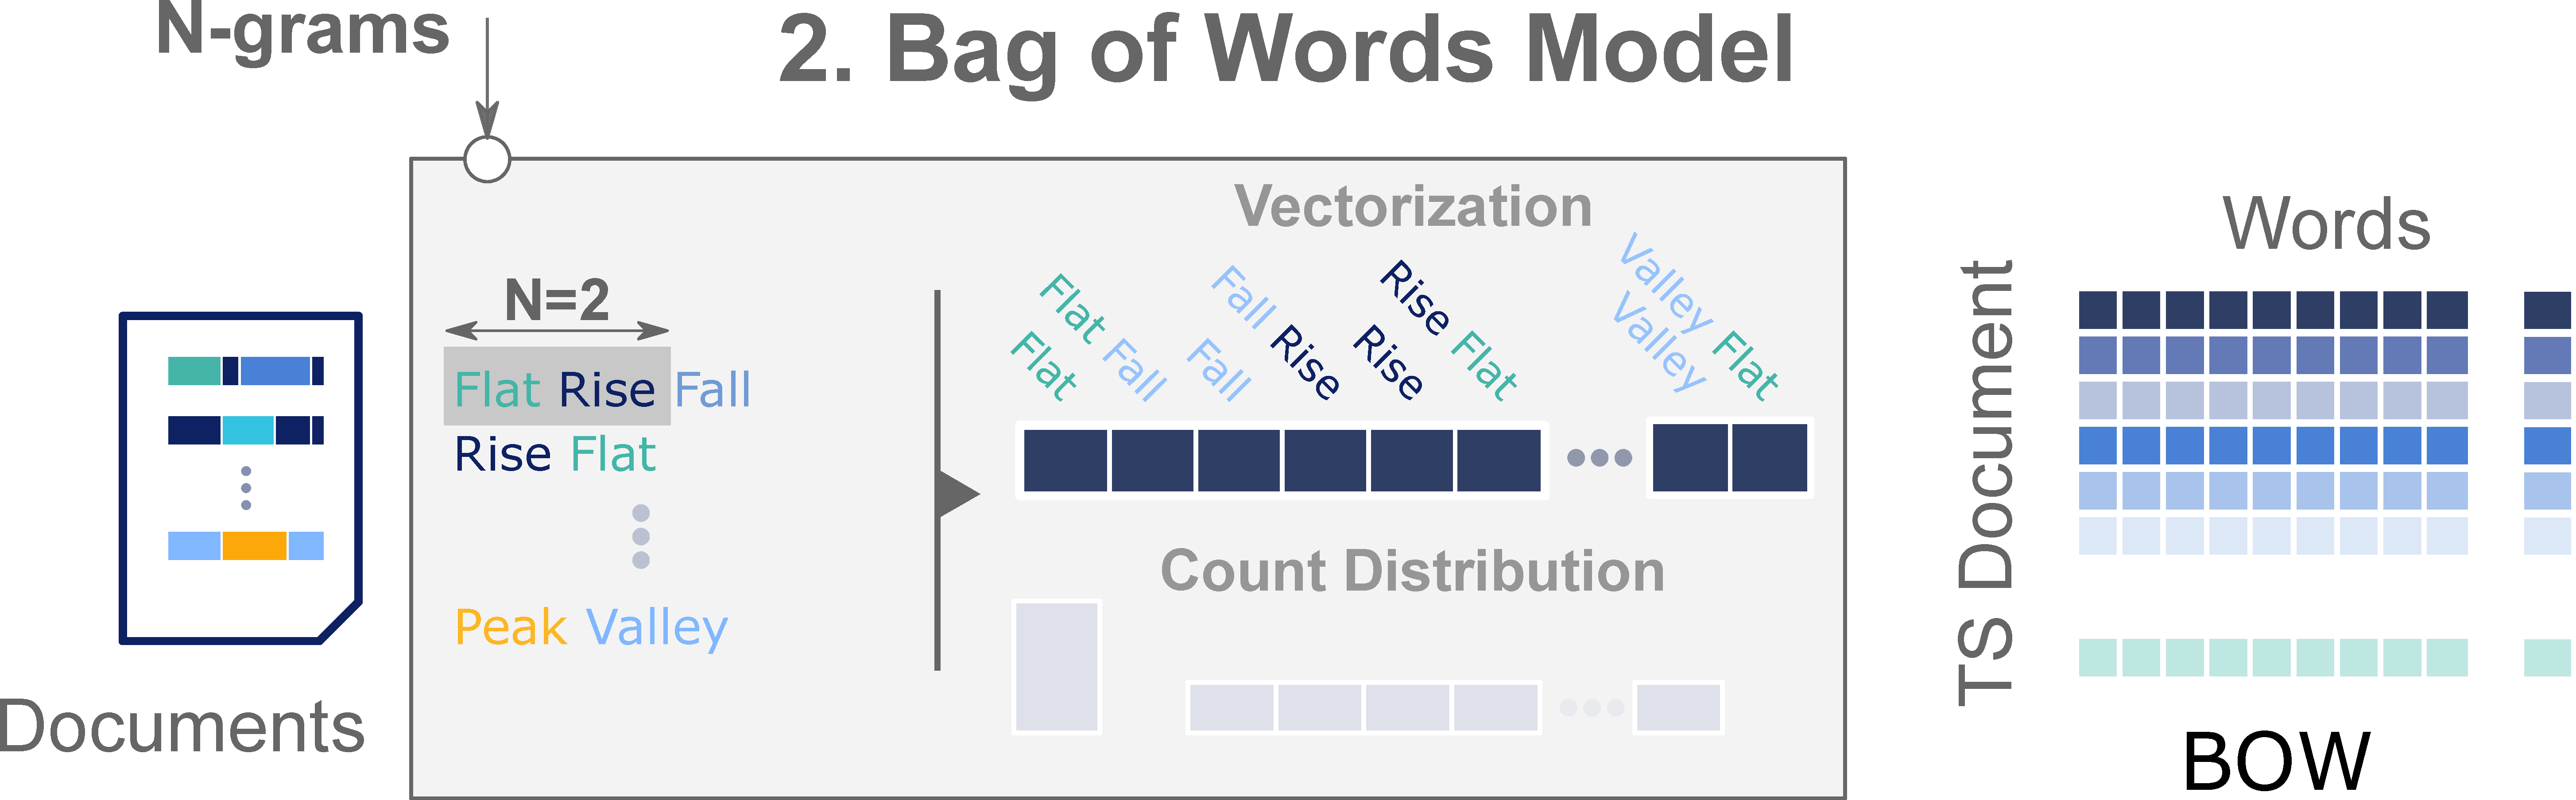
\includegraphics[width=\linewidth]{vectorization.pdf}
    \caption{Process to transform a time series document into a vectorized representation of words and n-grams. The user can set the size of the n-gram. The documents are transformed into the \gls{bow} having a count distribution, which is the \gls{tf}.}
    \label{fig:sentence_gen}
\end{figure}

The document generation stage receives a time series and transforms it into a \textit{document} with several sentences, descriptive of its shape and dynamics. As mentioned, this transformation is made with \gls{ssts}, which searches for specific patterns on a symbolic representation of the signal and for which a word is given.  
\par
After converting the time series into \textit{documents}, the text is analyzed to build a matrix of \textit{word} or \textit{n-gram} frequencies, the \gls{bow} model. In this case, the features extracted are purely statistical, but can provide a relevant measure of differences between documents. Each row of the \gls{bow} model is a time series \textit{document}, represented by columns that have the number of occurrences of a \textit{word} or \textit{n-gram}. Figure \ref{fig:sentence_gen} shows the vectorization of a time series \textit{document} as one row of the \gls{bow} model.

The \gls{bow} model can be used in several ways. Following guidelines from the text mining domain, it can be used for unsupervised or supervised tasks, for topic modeling and keyword extraction. The \gls{bow} model can also be trained with Naive Bayes Classifiers, Support Vector Machine or Linear Regressors \cite{scikit-learn}. In addition, the \gls{bow} model feature matrix can be converted into the \gls{tfidf} feature matrix, which can then be trained with the same classifiers. In this work, we explored several of these combinations to understand which can give better results.
\par
As was pointed out in Chapter \ref{cha:theory} (see Section \ref{subsec:text_features}), one of the reported issues of the \gls{bow} model is evaluating the relevance of a word based on its frequency in all documents, while not considering that words that occur in all documents might be less relevant. Therefore, we decided to use the \gls{tfidf} model, which increases the relevance of a word using its raw occurrences, while reducing its importance in proportion to the number of \textit{documents} that contain that word. The model is defined by being a ratio between the \gls{tf} and the \gls{idf} (equation \ref{eqn:tfidf}).

Both the \gls{bow} and \gls{tfidf} models give a weight to each \textit{word} for each \textit{document}. This means that each time series \textit{document} is vectorized into a distribution of weights for each \textit{word}, according to its presence on the time series \textit{document} and, in case of the \gls{tfidf} model, all the other time series \textit{documents}. The difference between the distribution of each \textit{document} can be used with a conventional distance measure to compare them. In Figure \ref{fig:distribution_dendogram} is showed the distribution of \textit{word's} weights for four different time series \textit{documents} of the \textit{Trace} dataset (see Section \ref{sec:dat_ucr}), based on a \gls{tfidf} model. The x-axis of each distribution is the \textit{word} or \textit{n-gram} and the y-axis, the corresponding weight for a time series document.
\par
The reader can notice that each distribution is different and this provides a way of distancing time series based on them. On the right of the distribution, the reader can see a dendrogram of sorting examples from the \textit{Trace} dataset. We used the cosine distance between vectors of time series documents (Symbolic Distance) and compared it with the \gls{ed}. Surprisingly, the \gls{ed} misses a few matches. Although the example is very simple, it highlights well how this strategy can compensate for some mismatches that can occur with the \gls{ed}.

\begin{figure}
    \centering
    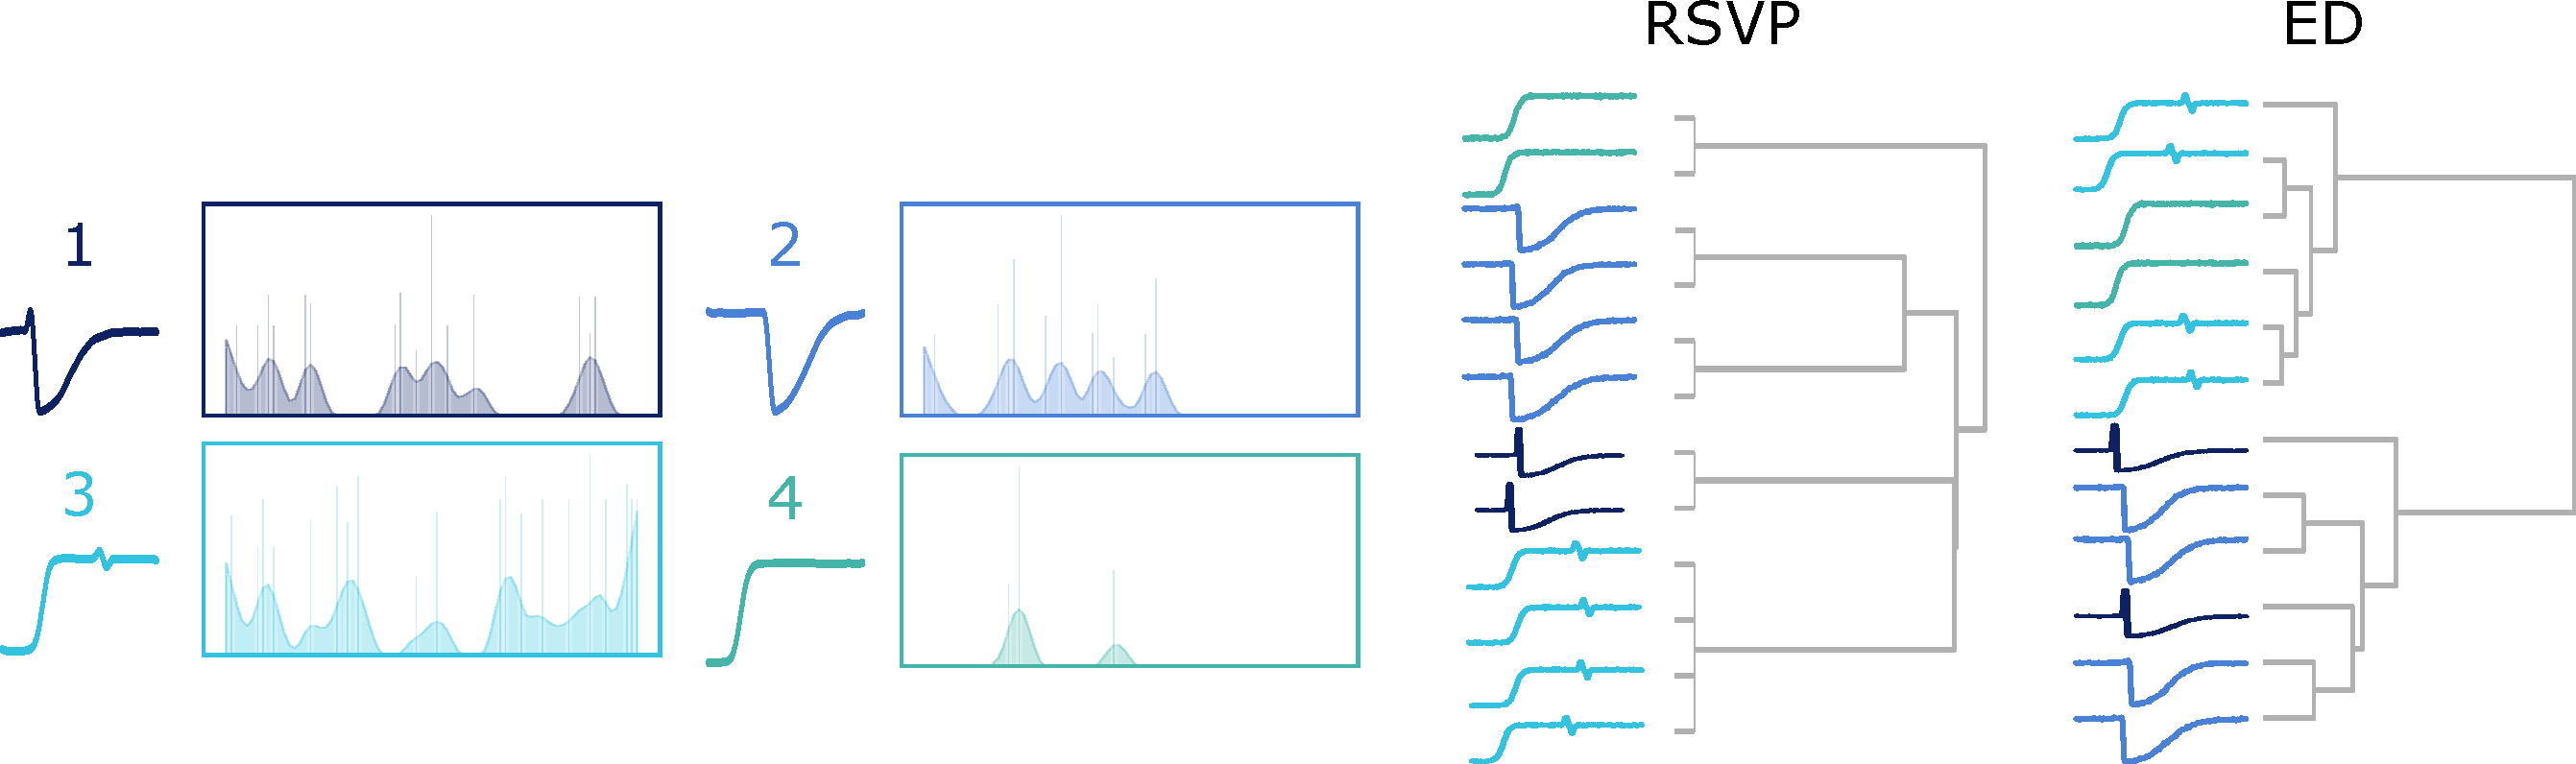
\includegraphics[width=\linewidth]{distribution_dendogram_ED_RSVP.pdf}
    \caption{Comparing the clustering process of the \gls{ed} and the proposed symbolic method (Symbolic Distance). In the proposed method, each signal has a word distribution vector, represented on the left. The signals are clustered based on these.}
    \label{fig:distribution_dendogram}
\end{figure}
 
As the reader can notice, the \gls{ed} mismatched signals from class 1 with signals from class 2, and signals from class 4 with signals from class 3. The fact that a misalignment between the main structures of the signals occur (the main peaks from signals of class 1 are misaligned and the main small peak and valley shapes of class 3 are slightly misaligned), increases the distance between signals that have the same shape. On the other end, the proposed strategy follows a distance measure based on the presence/absence of specific shapes, as well as how these are ordered (if \textit{n-grams} are used). This means that classes 1 and 2 will not be mismatched, because signals from class 1 have a peak whereas the ones from class 2 don't.

\subsection{Towards Interpretable Results}

Having demonstrated that it is possible to create a distance measure between time series with pure text, we highlight an advantage of working on the text domain, which is \textit{interpretability} of the data. By \textit{interpretability}, we mean that it is possible to extract meaning in what differentiates classes of signals. This advantage is taken because of the weighting factor attributed to each \textit{word} or \textit{n-gram} from the \gls{tfidf} model. As explained by Pavel Senin \textit{et. al}, the weights can be used as a weighting vector for each word extracted, highlighting the corresponding shape on the original signal and measuring its importance for the classification process \cite{sax_vsm}.

\begin{figure}
    \centering
    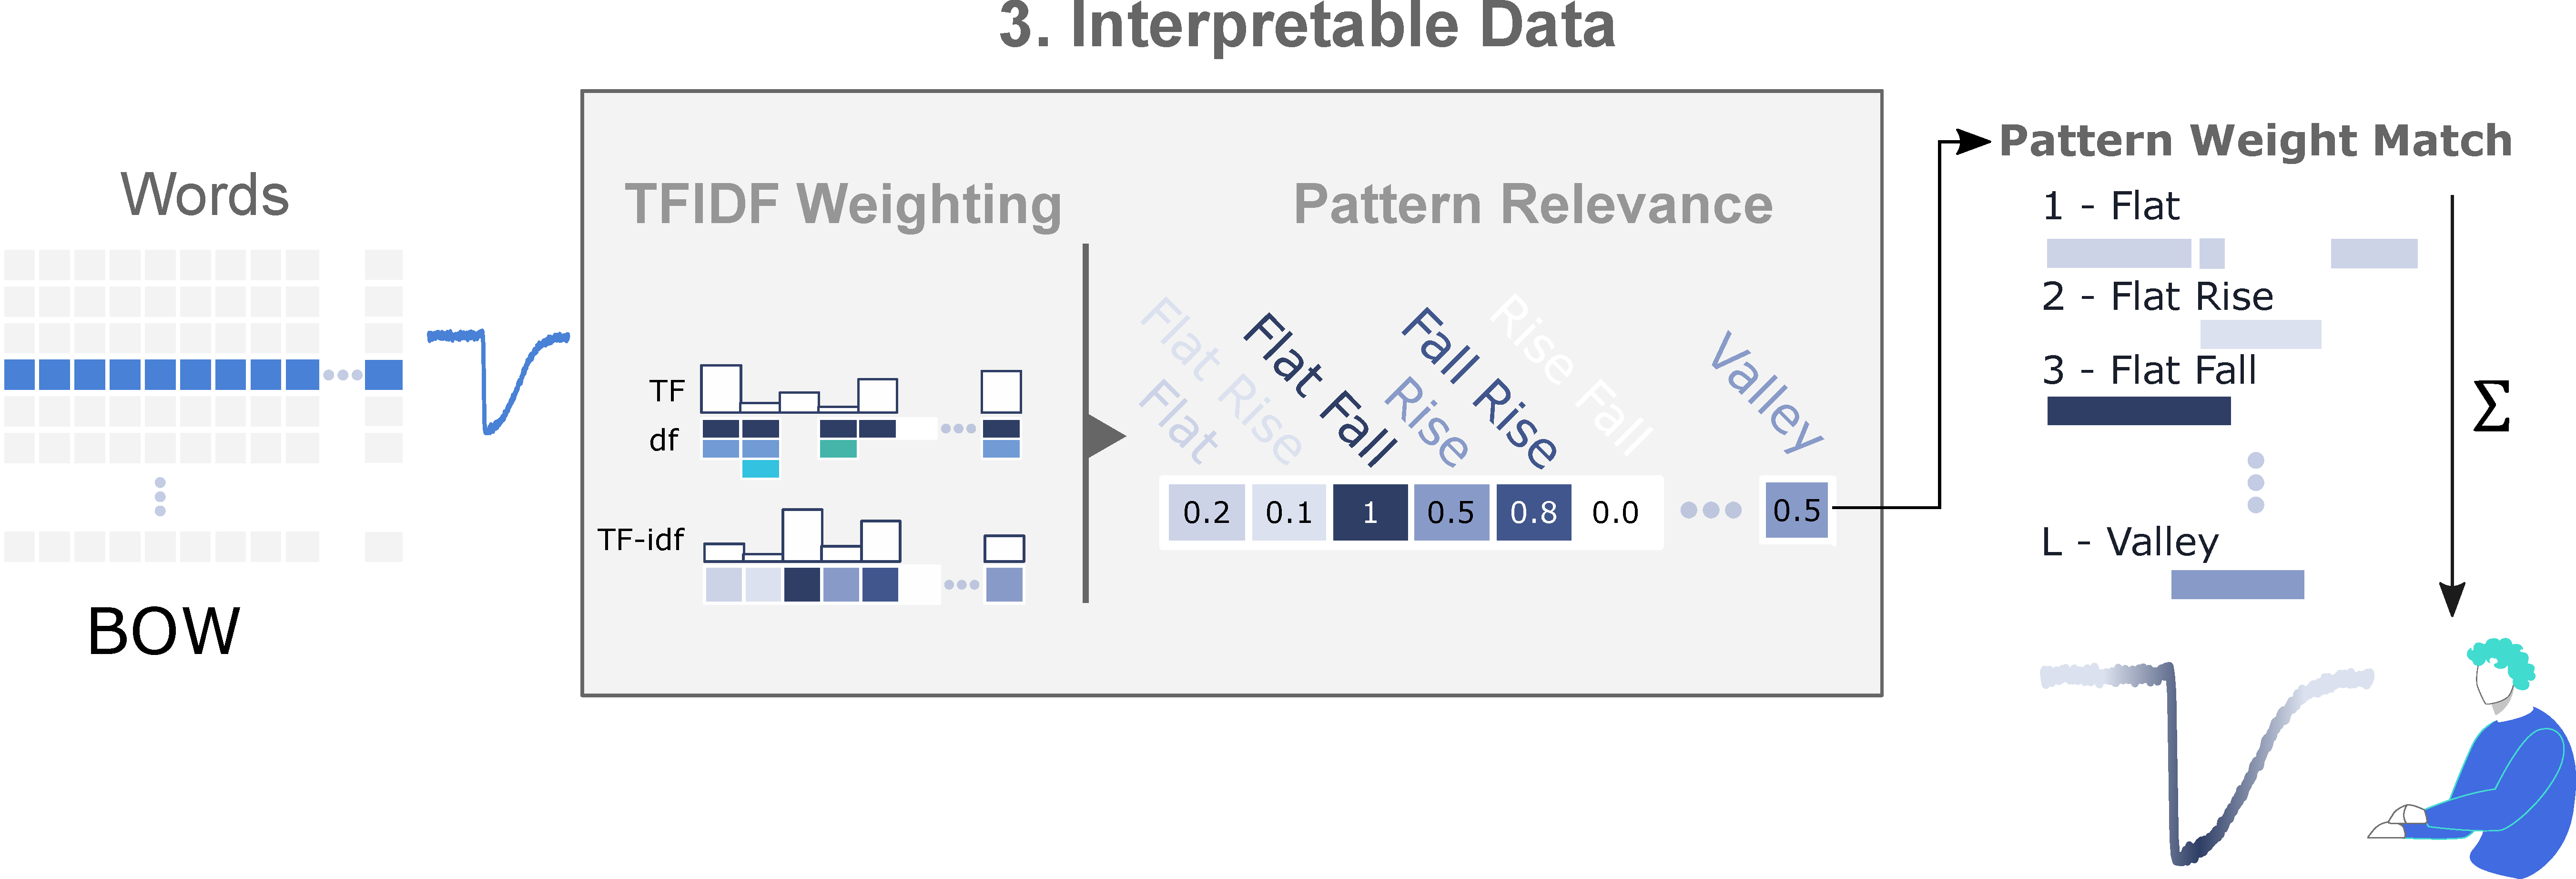
\includegraphics[width=\linewidth]{interpretable_scheme_explain.pdf}
    \caption{From the \gls{tfidf} matrix has weights for each word or n-gram (pattern relevance). The search of these words and cumulative attribution of weights on the segments matched can represent a feedback tool. In this case, the valley of the signal is highlighted.}
    \label{fig:interpretable_step}
\end{figure}


The process to highlight the areas of the signal that are more relevant and able to explain the difference between classes is illustrated in Figure \ref{fig:interpretable_step}. From the \gls{bow} model, the \gls{tfidf} model is computed, following equations \ref{eq:tf}, \ref{eq:idf} and \ref{eqn:tfidf}. From this representation, each \textit{time series} is represented as a vector of weights for each \textit{word}. These weights can be used to highlight the area of the signal represented by the corresponding \textit{word}. Therefore, the process is to search back the areas of the signal that match the \textit{word} or \textit{n-gram} ($w_i$) as an \gls{ssts} query, while keeping the corresponding \textit{weight} ($h_{ij}$), for word $i$ from time series document $j$, on the indexes of the match, with indexes $a$ and $b$:

\begin{equation}
(a,b) = ssts(t_j, w_i)
\end{equation}

In the end, the  weighted vectors are summed, returning a final vector ($WTS$) with the weighted contributions of all \textit{words}:

\begin{equation}
WTS_i(a, b) = WTS_i(a, b) + h_{ji}
\end{equation}

In Figure \ref{fig:interpretable_step}, the exemplified signal has a higher relevance on the \texttt{valley}, being the most characteristic element of that time series.

\section{Towards Natural Language for Pattern Search}

The fact that an analyst can search with \gls{regex} on time series makes the process more flexible and expressive and is innovative in the sense that text patterns can be written to search for specific shapes on a time series. In this journey to explore the topic of text-based queries for time series pattern search, we established the possibility of making an association between features and keywords to perform a search similar to what is done with web-searches toolbars. Thus, we propose a novel method, \gls{quots}, for pattern search, but in this case, it is based on natural language keywords and linguistic operators. In contrast with the previously explained method, \gls{ssts}, \gls{quots} associates \textit{words} with features, and such as \gls{ssts}, contributes to the democratization of pattern search on time series.

\subsection{Browsing Patterns Search}

When a user opens any search toolbar (such as \textit{Google}, \textit{Safari}, among others) and searches for a specific \textit{topic}, he/she will write a set of keywords that can match the \textit{topic} he/she is searching. The results of this process are a list of pages ranked based on how well they matched the \textit{keywords} used. Of course that in this example, search toolbars might have additional information, and not solely rely on the \textit{keywords} (maybe including geolocation, browser history, etc...) for the search process. However, let us take into account this simple \textit{keyword} based search process that we typically use when browsing the internet and apply it to pattern search on time series.

\begin{figure}
    \centering
    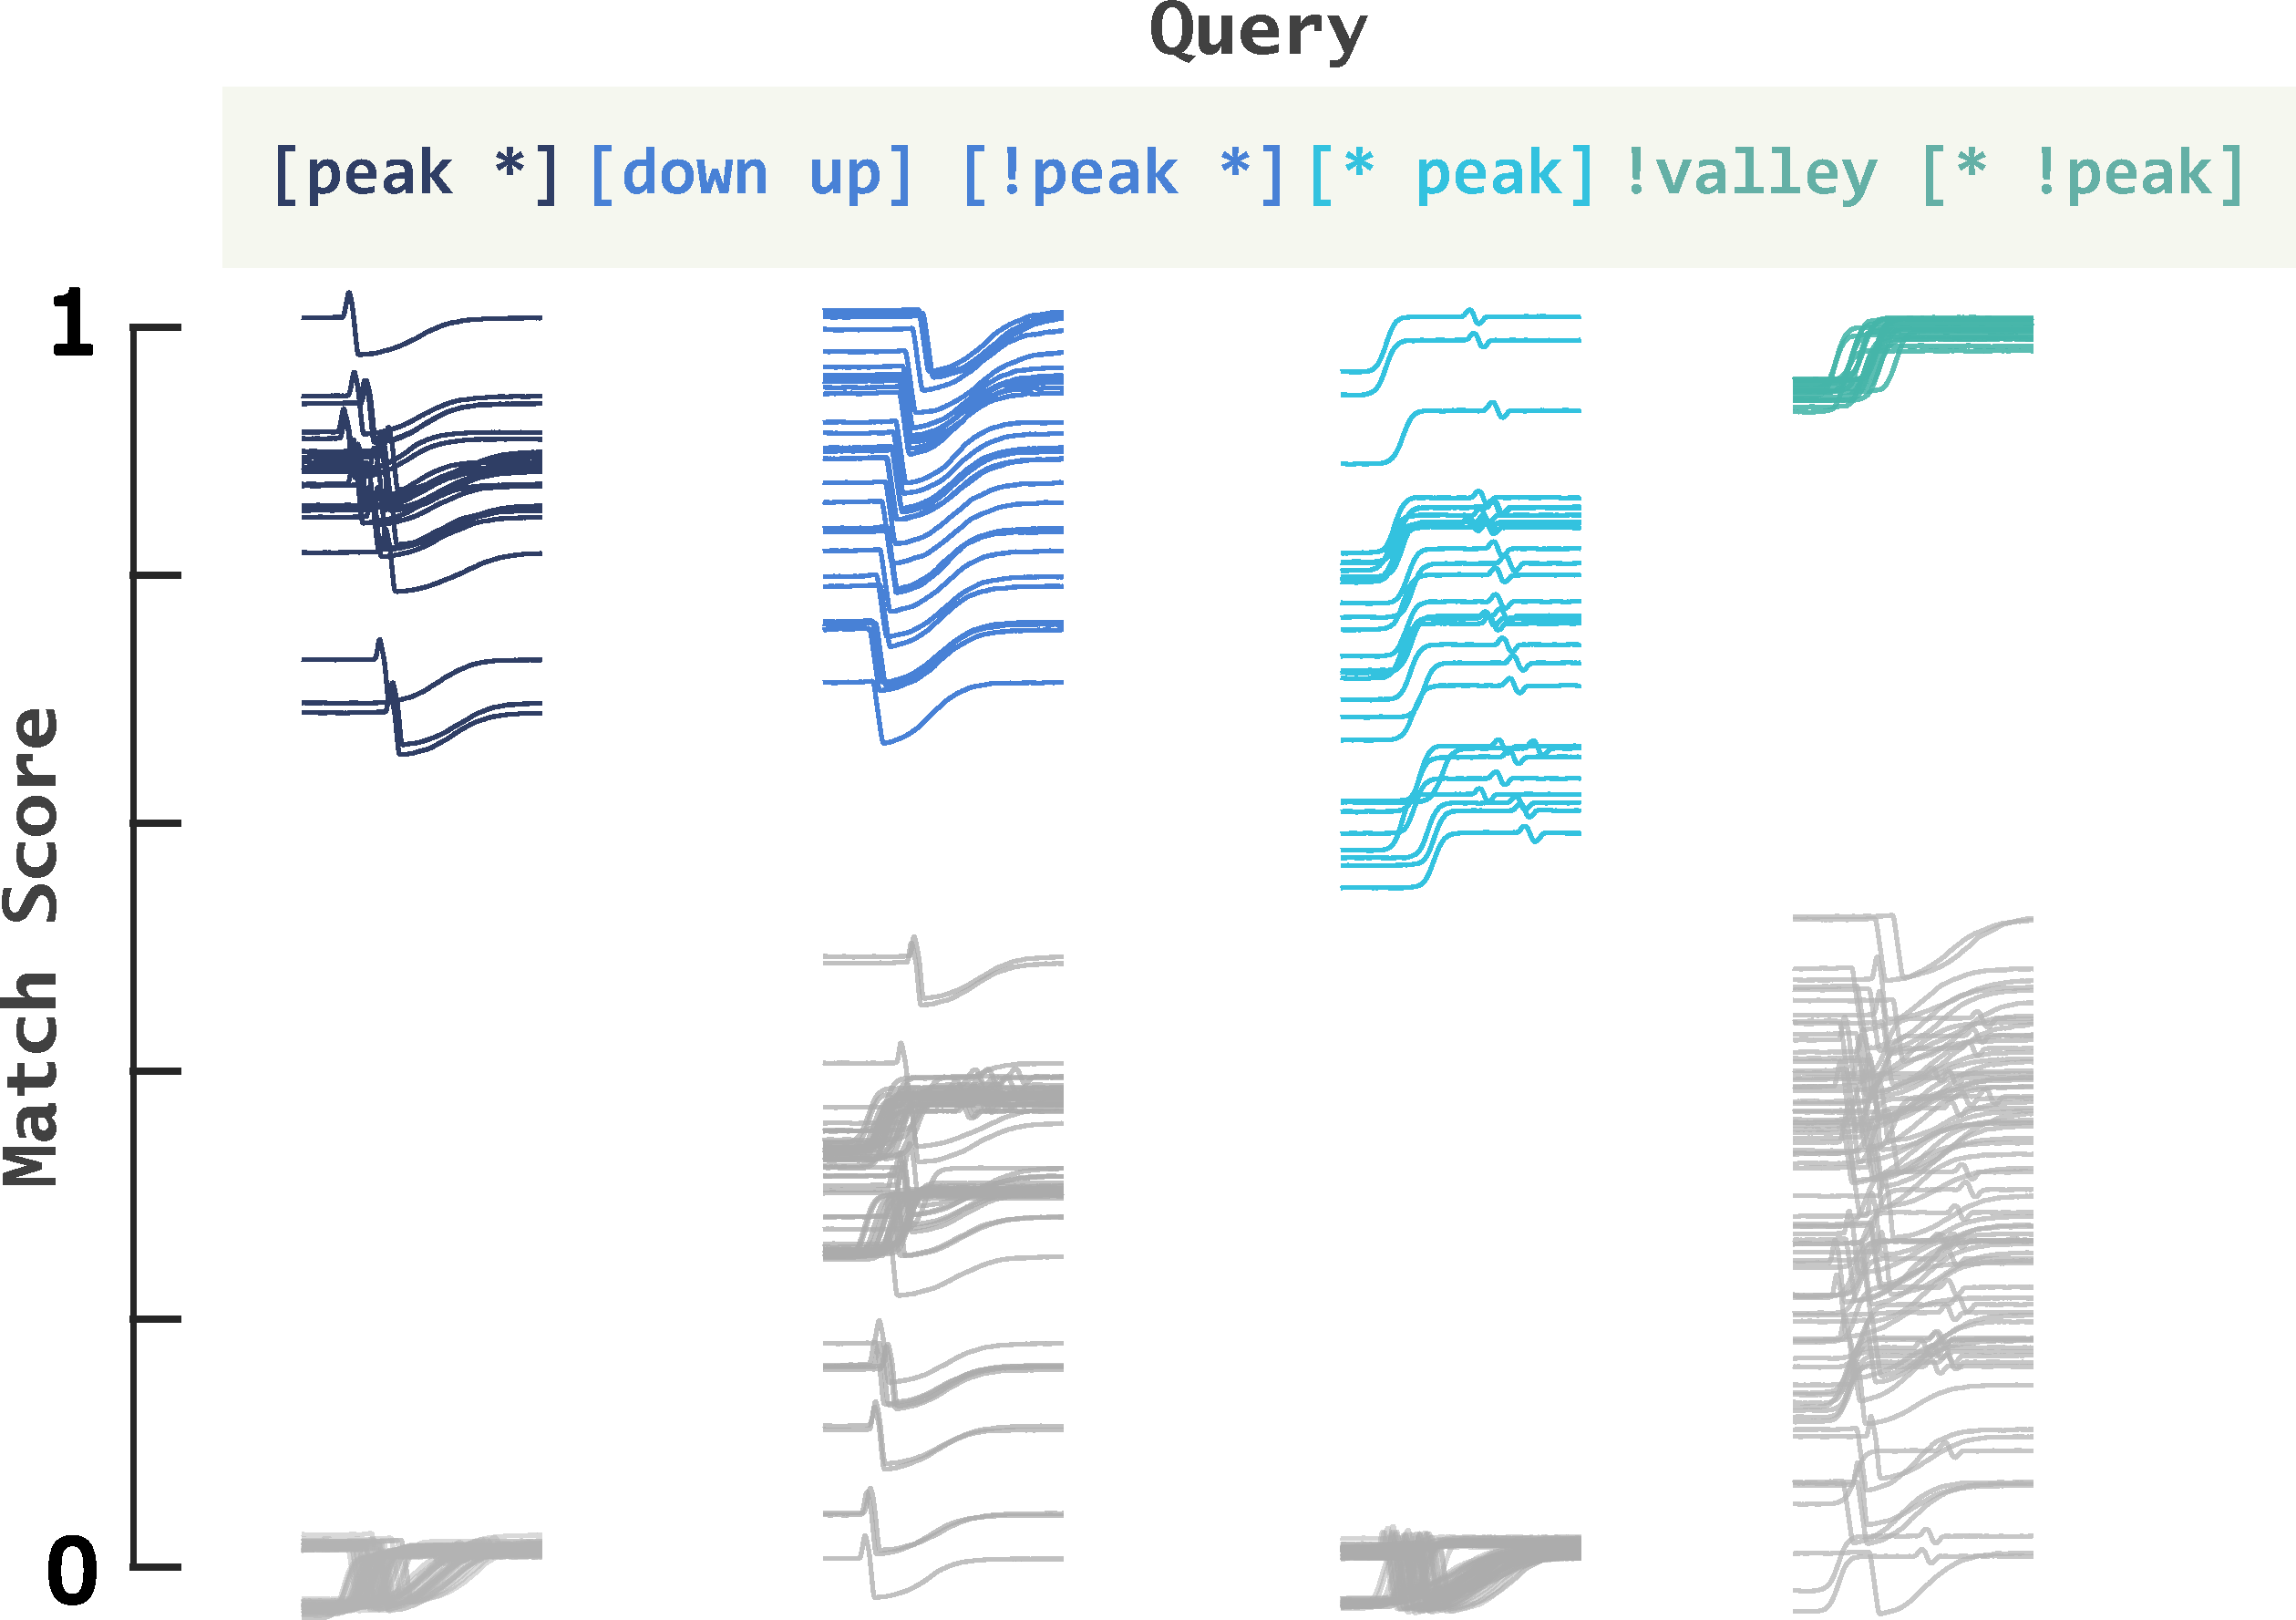
\includegraphics[width=0.85\linewidth]{quots_query.pdf}
    \caption{Using our proposed query language, we can create short, intuitive natural language queries to rank the 100 exemplars in Trace, separating our sought class from the remaining data. Here \texttt{*} is \textit{anything}, \texttt{!} is \textit{not}, and \textit{square brackets} are a grouping operator (more details in Section 3).}
    \label{fig:query_cold_start}
\end{figure}

As we mentioned above, patterns can be described with \textit{words} by associating text with specific properties or the presence of specific shapes on the pattern. In that sense, we propose to create a search paradigm that relies on words represented by features extracted from the signal. Informally, if a user wishes to find examples of a particular behaviour, he/she can simply \textit{Google it}, by describing the data he/she expects to see, given that behaviour. For example, we considered the four-class Trace dataset (see Section \ref{sec:dat_ucr}), which has been studied in more than 1,000 papers. As Figure \ref{fig:trace_quots_example} shows, it is possible to use our system to create queries that can separate each of the four classes from the rest of the data. This separation is possible simply by describing with \textit{words} the presence/absence of structures. Further, we will explain in detail how the process is done, which are the operators that we designed, and how queries can be written. Still, for now, we will explain the meaning of each query in this example. For instance, signals from class 1 (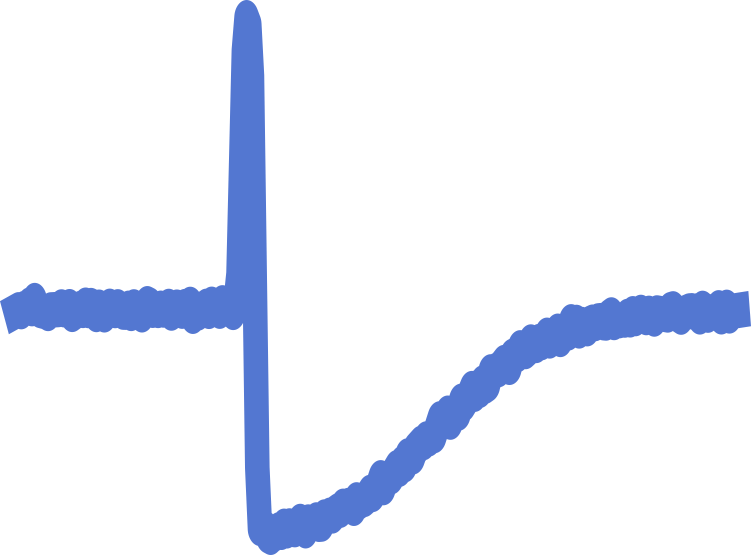
\includegraphics[height=2.5ex, width=3.5ex, valign=m]{trace1.png}) match well with query \texttt{[peak *]}, which translates into \textit{has a peak on the first half and anything on the second half}. The method sorts the signals based on this query and gives a very low score for all signals that do not have a peak in the first half of the signal. The same happens for the other queries, used to sort the other classes. A similar result is achieved with the inverse query \texttt{[* peak}, which means \textit{anything on the first half and a peak on the second half}, as well as the query \texttt{!valley [* !peak]}, which translates into \textit{has not a valley and has no peak on the second half}.

\begin{figure}
\centering
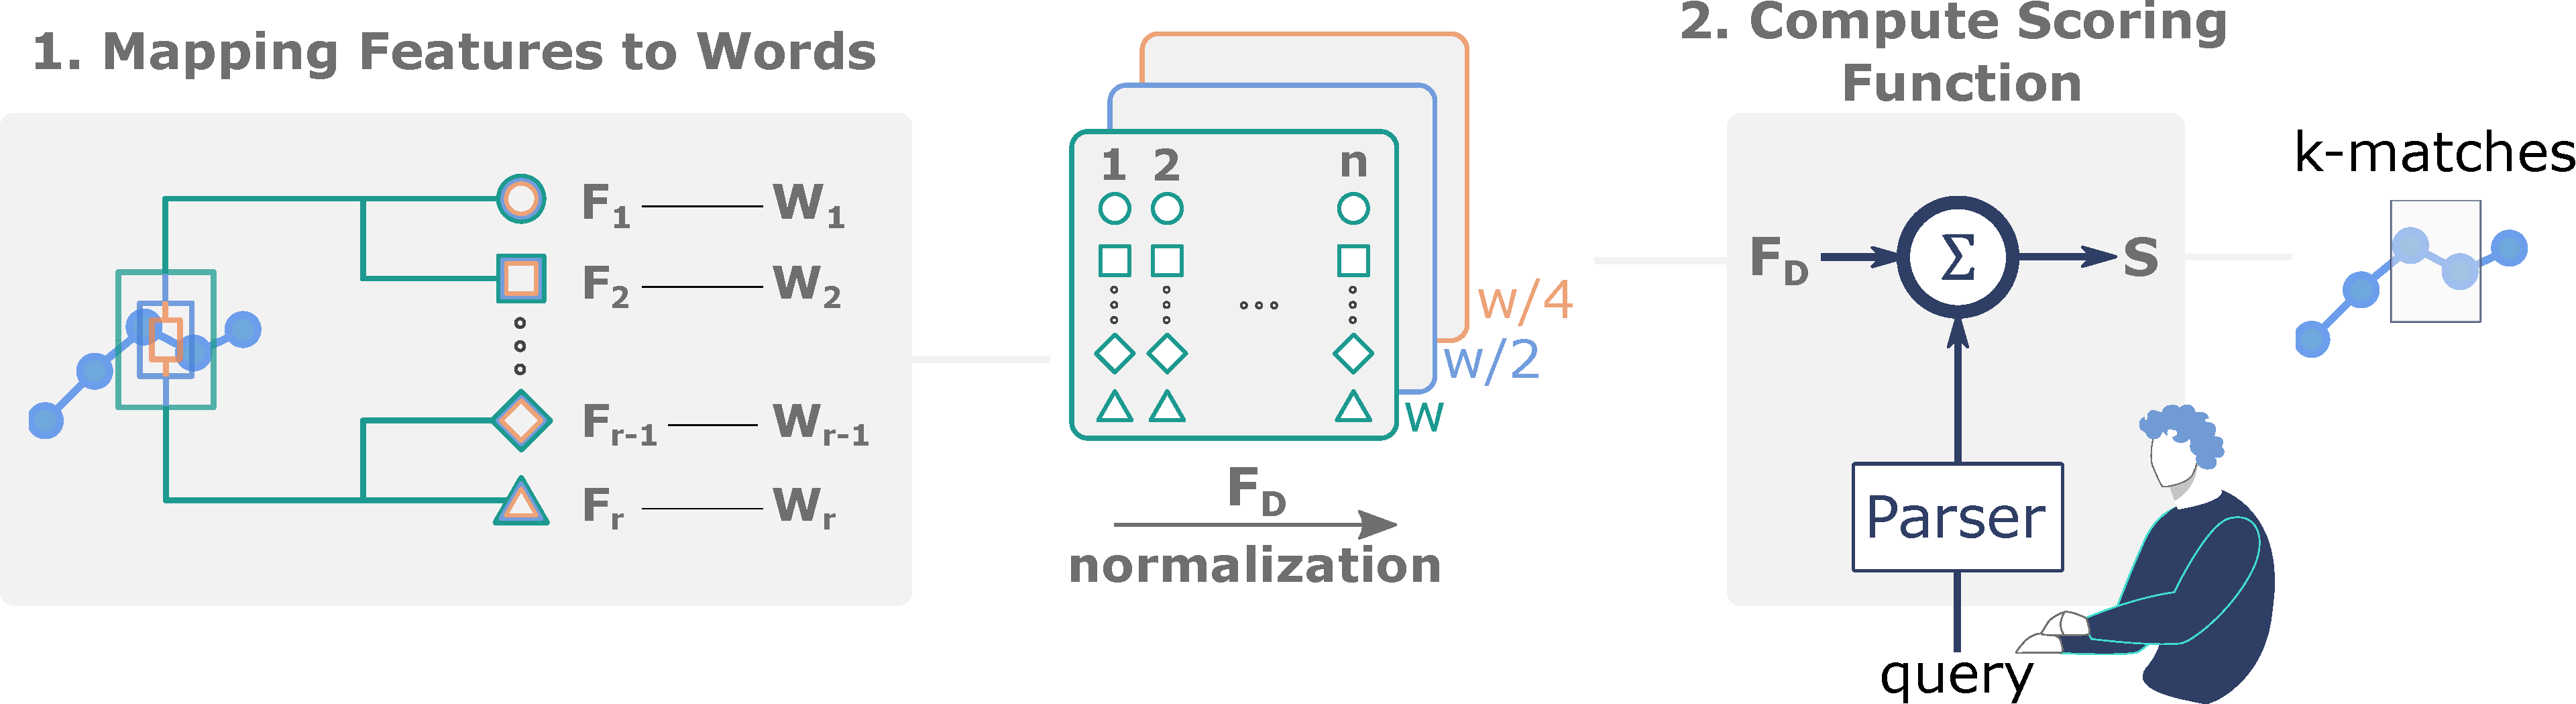
\includegraphics[width=\linewidth]{quots_steps.pdf}
\caption{\gls{quots} steps. It shows the feature extraction process and matches each feature to words ($W_1, W_2, etc...$). These features are computed in three window (\textit{w}) dimensions (\textit{w, w/2 and w/4}). The user can input a query to search for a specific pattern. This query will be scored based on the parser and features. It then returns the top \textit{k}-matches.}
\label{fig:quots_steps}
\end{figure}

The overall steps of the process are illustrated in Figure \ref{fig:quots_steps}. In order to perform the search with natural language keywords and operators, we represent the time series into a set of feature series. The features are extracted with a \textit{moving window}, with total overlap. The process is made three times, with decreasing window sizes (\textit{w}) dimensions (\textit{w, w/2 and w/4}). Each feature is associated with a \textit{word} ($W$) that should give a good intuition about the property it represents (e.g. \texttt{up} or \texttt{rising} should be clear to be indicative of the signal is rising). This feature set is the weight of the \textit{word} for each \textit{subsequence} of the signal. Such that when the \textit{words} are written, the features are summed according to the operators used. Then, the search returns the \textit{k-top} \textit{subsequence} matches for the query used.
\par
Concretely, with this method, we will demonstrate that the proposed natural language keyword representation is expressive enough to discriminate specific behaviours on a time series and that it moves towards a democratized time series analysis process, where analysts from other scientific domains, not familiar with programming languages, can also perform high-level pattern search.

\subsection{Mapping Features to Words}

We define a \textit{word feature vector} $W$ as a mapping of a feature series $F_i$ with a specific \textit{word} $W_i$. With feature, we intend to describe either a property, such as the mean or standard deviation, but also a distance measure to pre-defined examples. In linguistic terms, this \textit{word feature vector} is an adjective of the \textit{subsequence}. Every \textit{subsequence} $t_{i,m}$ from each time series $T$ is characterized by the selected set of \textit{words},  being created a set of \textit{word feature vectors} for each time series, further normalized between 0 and 1. The \textit{word feature vector} has the size of $T$ and the feature series values indicate how relevant is the \textit{word} in the \textit{subsequence}. Figure 3 shows an example of the word feature vectors for \textcolor{myblue4}{up (Fup)} and \textcolor{myblue3}{down (Fdown)}.

\begin{figure}[!h]
\centering
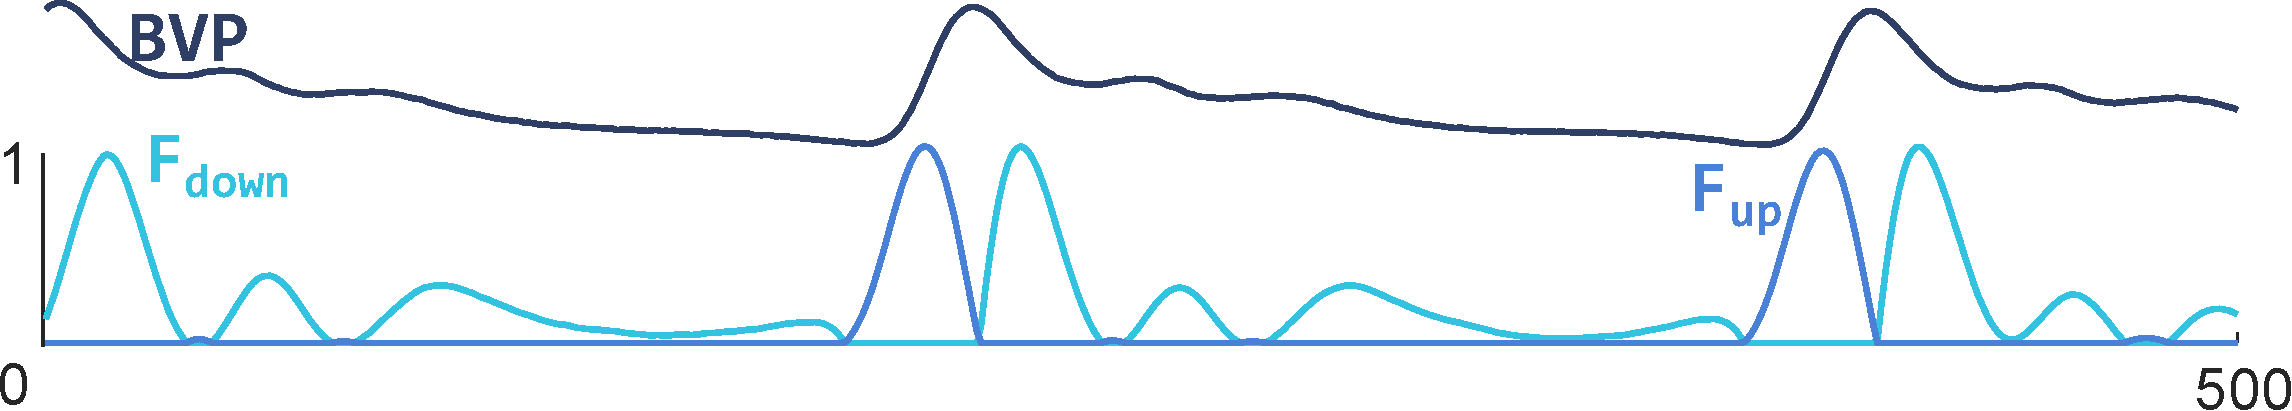
\includegraphics[width=\linewidth]{word_feature_vector.pdf}
\caption{Example of a word feature vector. In this case $F_{down}$ and $F_{up}$ represent a negative and positive slope value.}
\label{fig:wfv_example}
\end{figure}

To allow interactive search, the \textit{word feature vectors} are pre-computed in an offline indexing stage. In addition to this, we also extract three dimensions of the same word feature vector with different window lengths, based on $w$: $W_1 \rightarrow w$; $W_2 \rightarrow \frac{w}{2}$; $W_3 \rightarrow \frac{w}{4}$; with the intent of matching ordered sequences of words inside a subsequence with the \textit{grouped followed by} operator, as will be explained further. It is important to note that the ratio of the window used for the dimension $W_2$ and $W_3$ might have to be fine-tuned for the domain, as there might not be a “one window ratio fits all”. However, empirically we observed that the exact value of this ratio is not critical to the success of the search.

For each $W$ is assigned a \textit{word}. We use \textit{English} words to make the process more intuitive, such as \texttt{noise}, \texttt{up} and \texttt{peak}. We recognize that the intuitive meaning of such words can vary from user to user depending on their domain, their experience, and the current context. Either way, words can be mapped to features that are domain-specific or word feature vectors can be given a domain-specific vocable, providing a more appropriate mathematical thinking behind what is its meaning. In addition, we are aware that multiple words can be given the same meaning and for this reason, we associate several synonyms with each word.
\par
We define an initial subset of features that are mapped to words. When defining one \textit{word feature vector} it would often come with a negation pair. A negation pair ($!W$) represents the exact opposite of a defined \textit{word feature vector} ($W$) following the rule:

\begin{equation}
\label{eq:neg_pair}
!W = 1-W
\end{equation}

This indicates that when one increases the other one has to decrease proportionally. Examples of such \textit{word feature vectors} are \texttt{symmetric} and \texttt{asymmetric}, or \texttt{complex} and \texttt{simple}. Note that some words might be the opposite of each other, but do not follow this rule, or even seem to be the opposite of each other, but are not. For instance, \texttt{up} and \texttt{down} are opposite of each other, but do not follow Equation \ref{eq:neg_pair}. While one exists, the other can not, but it does not mean that when one is small, the other has to be high since the \textit{subsequence} might just be \texttt{flat}. Another case is the word \texttt{peak}. Intuitively, we would think that \texttt{valley} is the opposite of \texttt{peak}, but the consideration of \texttt{!peak = valley} (not being peak means it is a valley) is false. In this work, we use the negation of a word feature vector for cases where there is no negation pair. This negation is realized using an operator (See Table \ref{tab:operators}).
\par
As previously noted, a set of features is used to extract several properties of all \textit{subsequences} of a time series and attribute a semantic meaning to each one of them by mapping it to a specific \textit{word}. It is our assumption that a \textit{subsequence} can be mapped to a set of \textit{words} that an analyst would use to describe it. Depending on the domain or \textit{vocabulary} of the analyst, the set of words might have to be different and adjusted. Eventually, the \textit{dictionary} can be expanded to other types of \textit{features} and \textit{words}. In any case, we want to demonstrate that this current set of words and operators can solve many search problems with expressive queries.

\begin{table}
\begin{center}
\caption{List of all word feature vectors with examples. Here, $i \in [0,n]$, $n $ is the signal's size, $a$ is the beginning of the moving window, starting at $a=i-\frac{w}{2}$, and $w$ is the moving window size. The colors of the \textit{words} are the corresponding colors on the \textit{example}. Each example has representative feature vectors. When a negation pair is present, it is added to the example.}
\label{tab:operators}
\setlength{\tabcolsep}{3pt}
\begin{tabular}{L{0.2\linewidth}P M{0.15\linewidth}} 
\toprule[1.5pt]
Word & Description & Example\\
\toprule
\textbf{\texttt{\textcolor{myblue4}{Up}} (\textcolor{myblue3}{Down})} & The slope estimation of a linear adjustment ($y= ax + b$) to the \textit{subsequence}, being \texttt{up (down)} $= a$, if $a_{\texttt{up}}$>0 ($a_{\texttt{down}}$ <0) or \texttt{up (down)} $= 0$, if $a_{\texttt{up}}$<=0 ($a_{\texttt{down}}$ >=0) & 
\includegraphics[height=10ex, valign=m]{thumbnail_up_down.pdf}\\
\hline
\textbf{\texttt{\textcolor{myblue4}{Flat}}} & The inverse of the sum of absolute differences between the \textit{subsequence} and its average: \texttt{!flat(i)} $= \Sigma_{j=a}^{a+w} |t(j) - \overline{t(a,a+w)}|$. & 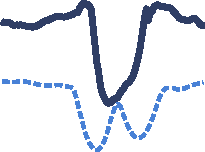
\includegraphics[height=10ex, valign=m]{thumbnail_flat.pdf}\\
\hline
\textbf{\texttt{\textcolor{myblue4}{Noise} (\textcolor{myblue3}{Smooth})}} & The residual error when modeled by a moving average ($ma$). \texttt{noise(i)} $=  \Sigma_{j=a}^{a+w} |t_j - ma_j|$. (\texttt{smooth} = \texttt{!noise}). & 
\includegraphics[height=10ex, valign=m]{thumbnail_noise.pdf}\\
\hline
\textbf{\texttt{\textcolor{myblue4}{Complex} (\textcolor{myblue3}{Simple})}} & The complexity-invariant distance measure of the \textit{subsequence} of \ref{eq:complexity}. (\texttt{simple = !complex}) & 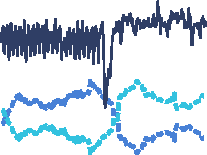
\includegraphics[height=10ex, valign=m]{thumbnail_complex.pdf}\\
\hline
\textbf{\texttt{\textcolor{myblue4}{Symmetric} (\textcolor{myblue3}{Asymmetric})}} & The normalized \gls{ed} (\ref{eq:norm_ed}) to the \textit{subsequence}’s horizontally flipped self. & 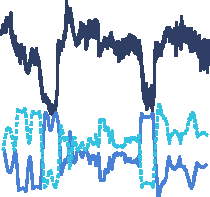
\includegraphics[height=10ex, valign=m]{thumbnail_symmetric.pdf}\\
\hline
\textbf{\texttt{\textcolor{myblue4}{Peak} (\textcolor{myblue3}{Valley})}} & The logarithmic normalized \gls{ed} (\ref{eq:norm_ed}) to the template of a peak (valley), modulated by a gaussian function. & 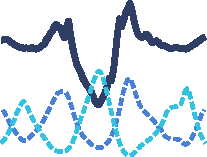
\includegraphics[height=10ex, valign=m]{thumbnail_valley_peak.pdf}\\
\hline
\textbf{\texttt{\textcolor{myblue4}{StepUp} (\textcolor{myblue3}{StepDown})}} & The logarithmic normalized \gls{ed} (\ref{eq:norm_ed}) to the template of a step-up(down) function. & 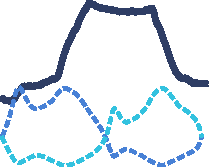
\includegraphics[height=10ex, valign=m]{thumbnail_step_up_down.pdf}\\
\hline
\textbf{\texttt{\textcolor{myblue4}{PlateauUp} (\textcolor{myblue3}{PlateauDown})}} & The logarithmic normalized \gls{ed} (\ref{eq:norm_ed})to the template of a plateau-up(down) function & 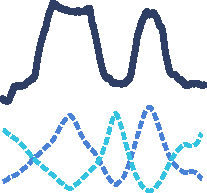
\includegraphics[height=10ex, valign=m]{thumbnail_plateau_up_down.pdf}\\
\hline
\textbf{\texttt{\textcolor{myblue4}{Top} (\textcolor{myblue3}{Bottom})}} & The moving average of the time series: $ma(i) = \frac{1}{w}\Sigma_{j=a}^{a+w} t(j)$. (\texttt{bottom = !top}) & 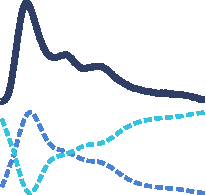
\includegraphics[height=10ex, valign=m]
{thumbnail_top_bottom.pdf}\\
\hline
\textbf{\texttt{\textcolor{myblue4}{High} (\textcolor{myblue3}{Low})}} & The difference between the maximum and minimum value of a \textit{subsequence}: \texttt{high(i)} $= max(t(a,a+w)) - min(t(a,a+w))$. (\texttt{low = !high}) & 
\includegraphics[height=10ex, valign=m]{thumbnail_high_low.pdf}\\
\hline
\textbf{\textit{Shape}} & The normalized \gls{ed} profile of the time series with a query (e.g. in orange) given by the user as an example. A word must be given as well and integrated into the query language. & 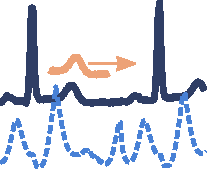
\includegraphics[height=10ex, valign=m]{thumbnail_shape.pdf}\\
\bottomrule[1.5pt]
\end{tabular}
\label{tab:quots_wfv}
\end{center}
\end{table}


\subsection{Linguistic Operators}

In the same way, we use word and sentence connectors in our language to create contrast or attribute a temporal sequence, in our proposed system we use \textit{operators}. An operator is a metacharacter or a word that can be used to diversify the way word feature vectors are handled, either in the way the information is extracted or how these are combined.  It contributes to a more versatile and expressive usage of this language. Currently, we have a simple list of four operators: \textit{negation} (\texttt{!}), \textit{wild card }(\texttt{*}), \texttt{followed by}, and \texttt{grouped followed by} (e.g., [$W_1 W_2 … W_w$]. This list can be expanded and customized, but we want to demonstrate that with a minimal set of operators, most of the problems we present are solvable. 

Web search engines have many operators at the user’s disposal, but since a list of words is usually powerful enough to retrieve and correctly sort most of the desired results, very few (or none!) are often used. We believe that this is the case for this application as well but acknowledge that simple operators can make the query more natural and come in handy to perform conjunctions between features and multiple dimensions, such as \textit{temporal logic} or \textit{negation}. For instance, we often rely on \textit{temporal logic} to express the presence of a shape in regards to another: \texttt{the peak that comes after the valley}, or even use the absence of a property: \texttt{it does not have a peak}. We also typically express the order in which structures occur on a time series: \texttt{up and then down}. These operators are especially useful to close the gap between the query and human discourse, contributing to a more expressive mechanism when using the proposed language. Currently, four operators are available. Below is a list and description of each of them, starting with the negation operator.
\par
\begin{itemize}

\item \textbf{Negation Operator  - \texttt{!W}} : As mentioned above, most words come as an opposite pair, but some do not follow Equation \ref{eq:neg_pair}. In these cases, or when the word has no direct opposite, it can be useful to penalize the presence of the word in a \textit{subsequence}. This operator does that by applying Equation \ref{eq:neg_pair} to the word feature vector, $W$. 

When describing time series, we inevitably use temporal logic in explaining the sequence of shapes we perceive. The next operator is \texttt{followed by}.
 
\item \textbf{\texttt{A followed by B}}: This operator rewards a \textit{subsequence} represented by A followed by one \textit{subsequence} that has a high score for B, within a distance of size $w$. A and B can be single words, multiple words, or even queries for different dimensions of the time series.

With this operator, we look ahead of a \textit{subsequence} in the time series. However, in some cases, it might be useful to describe the sequence inside the limits of the window we defined. For these, we have a special case of \texttt{followed by}, which is the \texttt{grouped followed by}, represented by square brackets ([ ]). 

\item	\textbf{Grouped \texttt{followed by} - [$W_1 W_2 … W_N$]}: Instead of looking ahead in the time series, we look inside the \textit{subsequence} to reward an ordered sequence of words. In this special case, the \textit{subsequence} is segmented into $N$ sub-windows, with size integer of $\frac{N}{m}$, and the corresponding \textit{word} is scored within this sub-window. For this, we use the other two dimensions of the word feature vectors ($W_2$ and $W_3$). If $N<=3$, $W_2$ is used, while if $N>3$, $W_3$ is used.

Often, within a \textit{subsequence}, the differentiating property occurs on the first half, last third or another sub-window of the \textit{subsequence}, while the remaining sub-window(s) is(are) not relevant. We, therefore, introduce the wildcard (\texttt{*}) operator.

\item \textbf{Wildcard - *:} The sub-window where * is used is valued equally for all \textit{subsequences}.
\end{itemize}

As with vocabulary, the reader could imagine expanding our dictionary of operators, but even with a limited set of them, we can successfully solve all the proposed search tasks, which cover dozens of examples. After presenting the set of elements that can be used in the proposed method to query a pattern of interest, we are ready to explain how the query is turned into a score function and finally how the selection of the \textit{k}-most relevant \textit{subsequences} is done. 

\subsection{Natural Language Query for Time Series}

As illustrated on Figure \ref{fig:quots_steps}, the user inputs a query with all the \textit{words} and \textit{operators} available. The query is parsed to calculate a matching score ($S$) that indicates which \textit{subsequences} are better represented by the query. The score is calculated based on the word features vectors extracted from the time series that are \textit{called} by the query.
\par
As mentioned, considering the possibility of using the \texttt{grouped followed by} operator, each feature is extracted three times with different window sizes. For each word, three sets of word feature vectors are stored ($W_1, W_2 and W_3$) based on the original window size ($w, \frac{w}{2} and \frac{w}{3}$). These word feature vectors are stored together in a \textit{dataframe} and called based on the \textit{word} written by the user. It is important to mention that all words are stored in a vocabulary file, associated with a \textit{thesaurus} file for synonym checks.
\par
If the signal is multidimensional, all three sets of \textit{word feature vectors} are extracted for each dimension. Having this set of information pre-computed helps make the search run at interactive speeds, even for large data collections. When all data is pre-computed, \gls{quots} is ready to accept queries by the user. 
\par
The query field accepts any word available in the vocabulary and \textit{thesaurus}. When any of the words are not present in our vocabulary, we alert the user which is the closest word available, based on \textit{edit distance}. The query can accept operators and works for multidimensional querying. These are relevant elements that are used as a reference to parse the query into individual scoring elements. This parsing process is made by looking into: (1) which dimension(s) of the time series is (are) included; (2) which operators are used; and (3) the single written words. The first two define how the score is calculated, that is, how word feature vectors are combined, as well as which dimensions of the word feature vectors are used. For instance, when including multiple signals, the query parses which word(s) corresponds to which signal, to search for the correct index of word feature vectors in the pre-computed \textit{dataframe}. To identify the signal, the following \gls{regex} is used to find all signal names \textit{\textbackslash w+:} (\textit{one or more characters ending with ":"}).


\begin{figure}
\centering
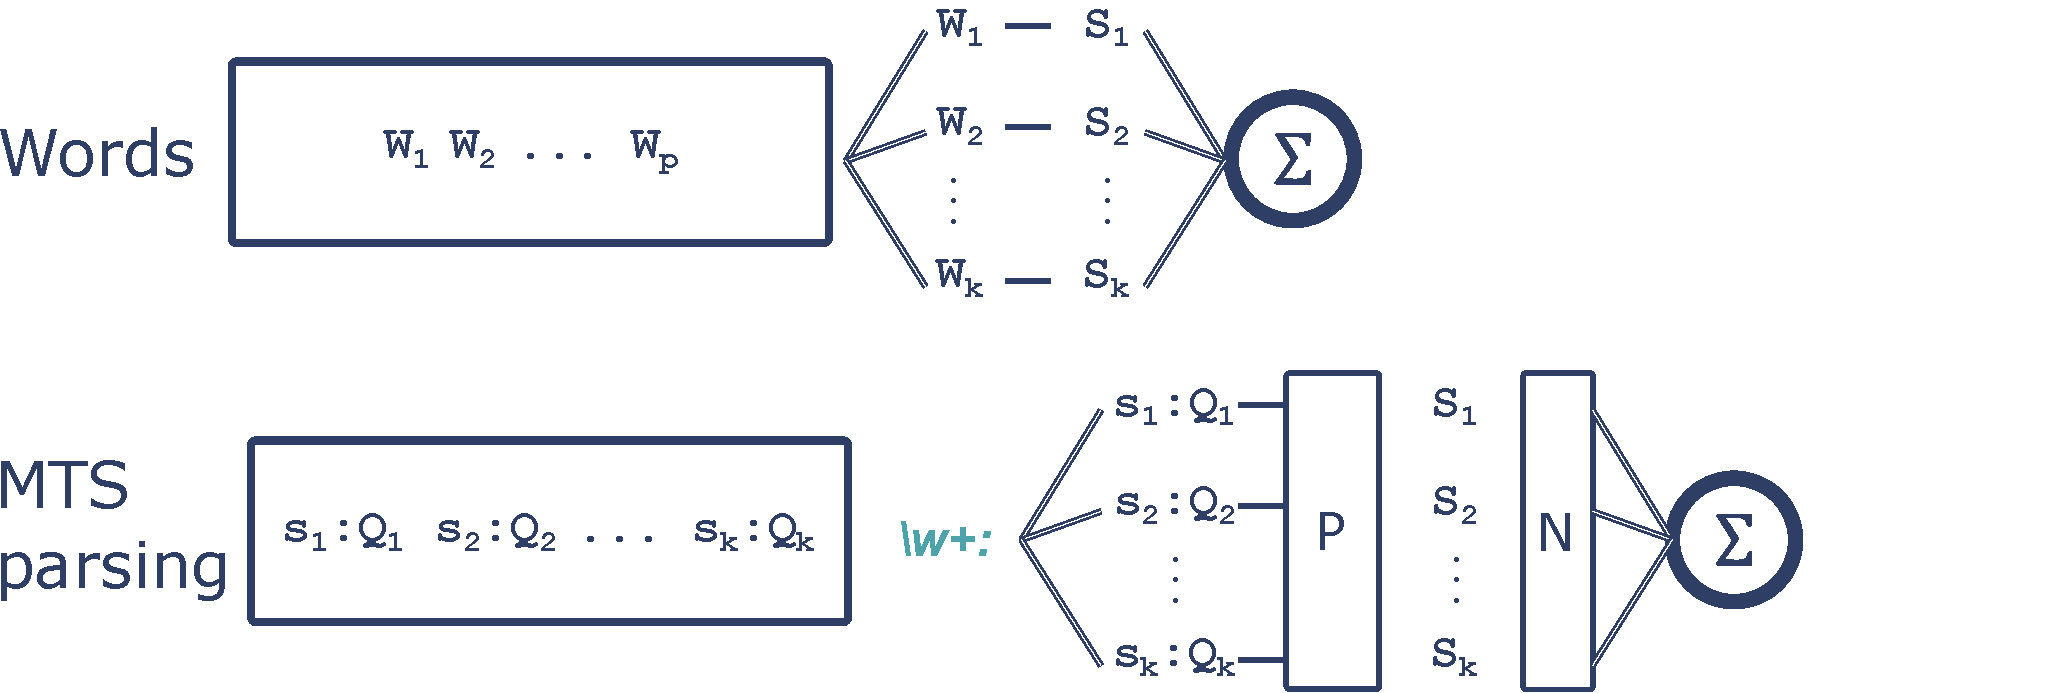
\includegraphics[width=\linewidth]{parser1.pdf}
\caption{Process to parse the input text query. When having simple space separated words, each corresponding word feature vector is summed together. When in multidimensional mode, there is the \textit{signal id} first.}
\label{fig:parser1}
\end{figure}

\begin{figure}
\centering
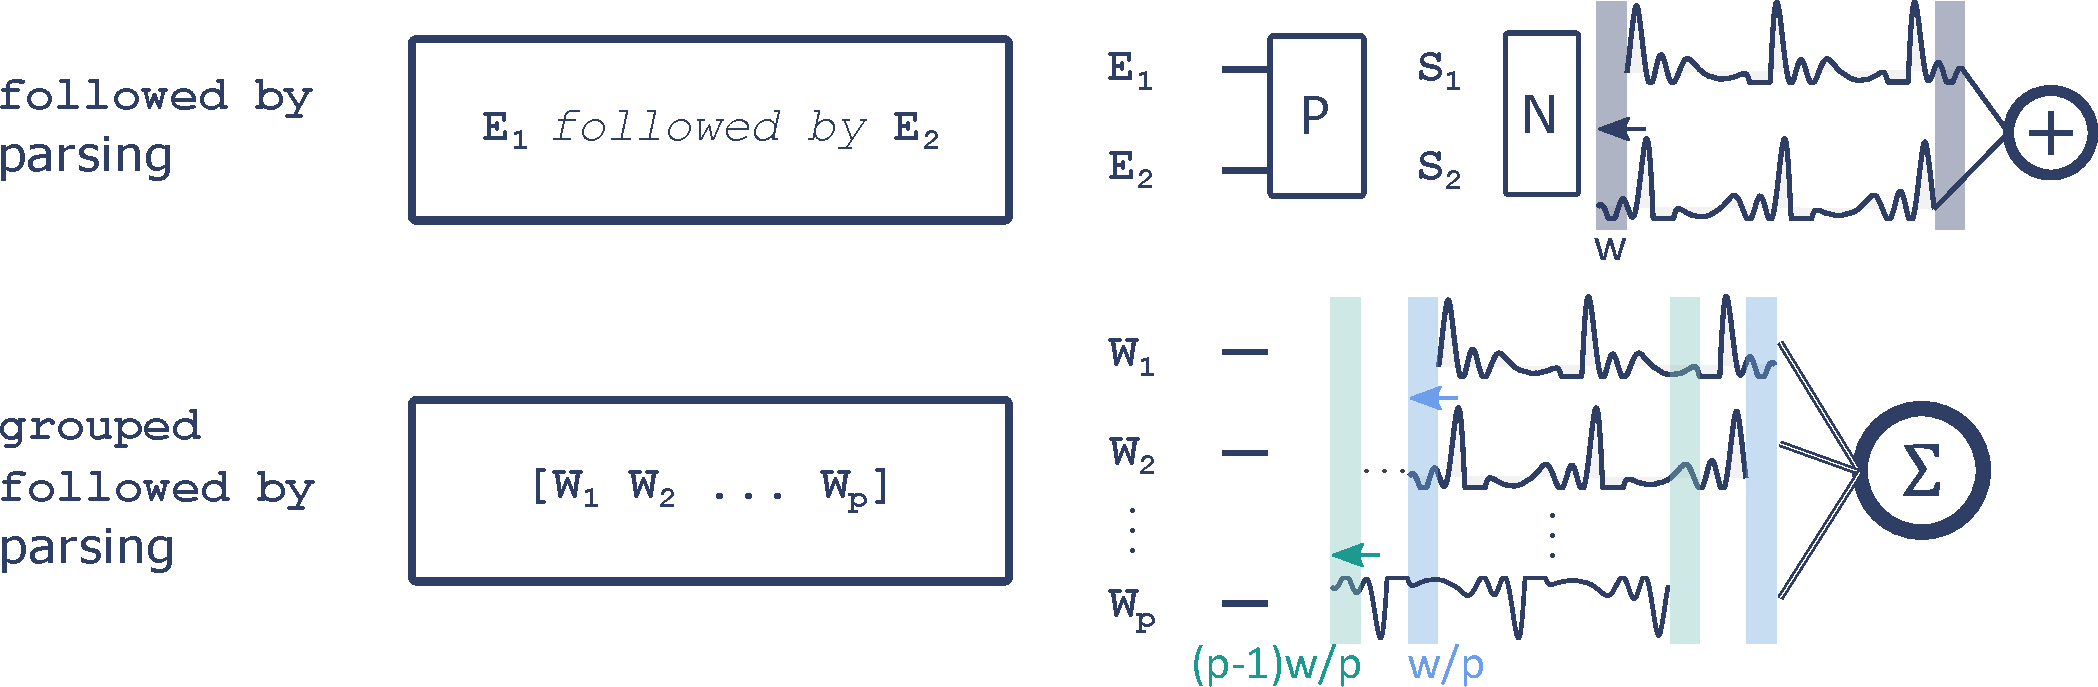
\includegraphics[width=\linewidth]{parser2.pdf}
\caption{Second order of the parser. In case the \texttt{followed by} operator is used, the elements ($E_1$ and $E_2$) are parsed (P) and word feature vectors are summed, but the $E_1$ has to be delayed to count as the "previous" instance ($w$ represents the selected window size). When using the more specific \texttt{grouped followed by} operator, square brackets are used and represent the window size highlighting the signal. Only words can be used in these brackets and are added together, delaying each word based on their position inside the brackets, for instance, word 2 ($W_2$) is delayed by the window size, divided by the number of words inside the brackets (w/p).}
\label{fig:parser2}
\end{figure}

When the \texttt{followed by} operator is used, the query is parsed in the \textit{elements} that come before and after it (this is applicable either if the operator is used for intra-signal or inter-signal search). For this, the following \gls{regex} is used to separate the \textit{words} before and after the operator: \textit{\textbackslash w+ followed by \textbackslash w+} (\textit(word or words before followed by and word or words after it). What is meant by \textit{elements} is either \textit{words} (intra-signal) or two different signal dimensions (inter-signal). Another temporal operator is the \texttt{grouped followed by}, which is parsed by identifying square brackets in the query with the following \gls{regex} \textit{\textbackslash[.+?\textbackslash]} (\textit{anything inside square brackets}). The content of the square brackets is then combined (see Figure \ref{fig:parser2}).

When any of these elements are parsed, we end up with a single word or sequence of words, which are combined by summing their corresponding \textit{word feature vectors} (this corresponds to an implicit OR). Figures \ref{fig:parser1} and \ref{fig:parser2} give a visual aid to understand the parsing process for each case.

The simplest case for a query would be a sequence of \textit{words}. In this case, each \textit{word feature vector},  associated with the corresponding \textit{word}, is a score ($S$) function and is summed together to give the final score. In case a multidimensional signal is used, the user can write a multidimensional query, identifying a specific query ($Q$) for each dimension ($s_1, s_2,...s_k$). For this, each query $Q$ corresponding to a signal $s$ is treated individually by the standard parser ($P$ on Figure \ref{fig:parser1}), resulting in a scoring function ($S$) for each signal used on the query. Before summing all scoring functions, these have to be normalized ($N$ on Figure \ref{fig:parser1}) to have equal weight. It is important to note that $Q$ can be a query with \textit{words} or the \texttt{grouped followed by} operator.

The temporal operators are parsed by the \gls{regex}, as mentioned above. From the \texttt{grouped followed by} operator, only \textit{words} can be used and are combined with a temporal delay that depends on the number of \textit{words} inside the brackets. The brackets represent the limits of the \textit{window} that is used to extract the \textit{word feature vectors}. In that sense, when using two \textit{words} inside the brackets, it is expected that the first half of the signal has the first word, and the second half has the second word. This is extended to additional words inside the brackets. In order to combine the \textit{word feature vectors} of the \textit{words} used inside the brackets, we delay each \textit{word feature vector} based on the number of \textit{words} and corresponding position inside the brackets, such that \textit{words} after the first one are delayed $\frac{(i-1)w}{p}$ samples, being $i$ the position inside the brackets, $p$ the total number of \textit{words} inside the brackets and $w$ the window size. The delayed vectors are added together. For example, if using the query \texttt{[up down]} and features were extracted by a window with size of 100 samples, the \textit{word feature vector} for the word \texttt{down} is delayed 50 samples and added to the \texttt{up} \textit{word feature vector}. When used in combination with individual \textit{words}, the scoring function resulting from this operator is normalized between [0-1]. The reasoning is that each segment of the query should be weighted the same (e.g., if using the query \texttt{noise [up down]}, as \texttt{up} and \texttt{down} are combined, the range of this segment is [0-2], while \texttt{noise} is [0-1]. Therefore, \texttt{[up down]} is normalized between [0-1] before being added to \texttt{noise}). A similar process is performed with the \texttt{followed by} operator. The scoring function for the query previous to the operator is added to the scoring function of the query next to the operator but delayed by one window size ($w$).
\par
Finally, depending on the \textit{words} and operators used, the resulting scoring function is used to search for the \textit{k}-top \textit{subsequences}. This is made by searching in \textit{k}-iterations the maximum value of the scoring function. During this iteration process, trivial matches are not considered. A trivial match is a high-valued sample of the scoring function that is a neighbor of the maximum value found. To avoid these matches, all samples of the scoring function around a \textit{k}-top match on the scoring function ([$argmax(S)-\frac{w}{2}, argmax(S)+\frac{w}{2}$]) are converted to $0$. The matched \textit{subsequences} are highlighted on the signal and sorted by their match score.